\chapter{Wavefunctions}
\section{Slater Determinant Wavefunctions}
\subsection{The Energy Expression}

Consider a wavefunction of the form
\begin{equation}
{\cal A} \left[ \psi_a (1) \psi_b (2) \cdots \psi_n (N) \right] = 
{\cal A} \Psi
\label{chap15-eqno1}
\end{equation}
where $\psi_i$ is a spin orbital, a function describing the spatial and spin 
coordinates of the electron, and $\Psi$ denotes the product of all $N$ spin 
orbitals.  In Chapter 5, we showed that it is no restriction to take 
the spin orbitals of (\ref{chap15-eqno1}) to be orthonormal
\begin{equation}
\langle \psi_i | \psi_j \rangle = \delta_{ij}
\label{chap15-eqno2}
\end{equation}
and we will do so throughout this section.

First, we need to evaluate the energy of (\ref{chap15-eqno1})
\begin{equation}
E = {\langle \Psi | {\cal H} | {\cal A} \Psi \rangle \over \langle 
\Psi | {\cal A} \Psi \rangle}
\label{chap15-eqno3}
\end{equation}
using the results of Chapter 5.  The denominator has the form
\begin{equation}
D = \langle \Psi | {\cal A} \psi \rangle = \sum_{\pi} \zeta_{\pi} 
\langle \Psi | \pi \Psi \rangle
\label{chap15-eqno4}
\end{equation}
Any interchange leads to overlapping orbitals and hence, since the
orbitals are orothogonal all terms in (\ref{chap15-eqno4}), other than
$\pi = e$, must lead to zero.  For example, for $\pi = (12)$, we
obtain
\begin{eqnarray}
\langle \Psi | \pi_{12} \Psi \rangle &=& \langle \psi_a \psi_b \psi_c 
\cdots \psi_n | \psi_b \psi_a \psi_c \cdots \psi_n \rangle\cr
&=& \underbrace{\langle \psi_a | \psi_v \rangle}_{0} 
\underbrace{\langle \psi_b | \psi_a \rangle}_{0} \underbrace{\langle 
\psi_c | \psi_c \rangle}_{1} \cdots \underbrace{\psi_n | \psi_n 
\rangle}_{1} = 0
\end{eqnarray}
Hence,
\begin{equation}
D = 1
\label{chap15-eqno5}
\end{equation}

\subsubsection{The One-Electron Terms}

Consider the term
\begin{equation}
\langle \Psi | h ( 1 ) | {\cal A} \Psi \rangle = \sum_{\pi} 
\zeta_{\pi} \langle | h ( 1 ) | \pi \Psi \rangle
\end{equation}
For example, with $\pi = (12)$ we obtain
\begin{equation}
\langle \Psi | h ( 1 ) | \pi \Psi \rangle = \langle \psi_a | h | 
\psi_b \rangle \underbrace{\langle \psi_b | \psi_a \rangle}_{0} 
\langle \psi_c | \psi_c \rangle \cdots \langle \psi_n | \psi_n 
\rangle = 0
\end{equation}
Any interchange, other than $\pi = e$, necessarily puts at least two orbitals 
out of alignment.  The one-electron operator $h(1)$ can lead to a nonzero 
integral between orthogonal orbitals $\langle \psi_a | h | \psi_b \rangle$.
However, there is also at least one other overlap between orthogonal spin
orbitals, leading then to a zero matrix element.  Thus,
\begin{equation}
\langle \Psi | h ( 1 ) | {\cal A} \Psi \rangle = \langle \Psi | h ( 
1 ) | \Psi \rangle = \langle \psi_a | h | \psi_a \rangle
\end{equation}
and the total contribution from the one-electron part of ${\cal H}$ is just
\begin{equation}
\langle \Psi \left| \sum_{i} h (i) \right| {\cal A} \Psi \rangle = \sum_{j} 
\langle \psi_j | h | \psi_j \rangle
\label{chap15-eqno6}
\end{equation}
the result would be obtained with the antisymmetrizer omitted.  Of
course, the antisymmetrizer has still played a big role in the
one-electron energy.  Namely, it told us to use orthogonal spin
orbitals.  If it were not for the Pauli principle and the concomitant
${\cal A}$ in (\ref{chap15-eqno1}), we could have placed all the
electrons in the $\psi_i$ with lowest energy, obtaining a much lower
one-electron energy.

\subsubsection{The Two-Electron Terms}

Next we examine the two-electron part of ${\cal H}$.  For example,
\begin{equation}
\langle \Psi \left| {1 \over r_{23}} \right| {\cal A} \Psi \rangle = 
\sum_{\pi} \zeta_{\pi} \langle \Psi \left| {1 \over r_{23}} \right| \pi 
\Psi \rangle
\end{equation}
Consider $\pi = (12)$, then
\begin{equation}
\langle \Psi \left| {1 \over r_{23}} \right| (12) \Psi \rangle = 
\langle \psi_a | \psi_b \rangle \langle  \psi_b \psi_c \left| {1 \over 
r_{23}} \right| \psi_a \psi_c \rangle \langle \psi_d | \psi_d \rangle 
\cdots
\end{equation}
This involves an overlap of orthogonal orbitals for electron 1 and hence, we
get zero.  The only $\pi$ leading to a nonzero integral are
\begin{equation}
\pi = e : \langle \Psi \left| {1 \over r_{23}} \right| \pi \Psi 
\rangle = J_{bc}
\end{equation}
and
\begin{equation}
\pi = (23) : \langle \Psi \left| {1 \over r_{23}} \right| \pi \Psi 
\rangle = K_{bc}
\end{equation}
All other permutations leads to an overlap between orthogonal orbitals.
Thus,
\begin{equation}
\langle \Psi \left| {1 \over r_{23}} \right| {\cal A} \Psi \rangle = 
J_{bc} - K_{bc}
\end{equation}
Considering the other two-electron parts of ${\cal H}$, we obtain
\begin{equation}
\langle \Psi \left| \sum_{i>j} {1 \over r_{ij}} \right| {\cal A} \Psi 
\rangle = \sum_{i>j} \left( J_{ij} - K_{ij} \right)
\label{chap15-eqno7}
\end{equation}
Combining (\ref{chap15-eqno5}), (\ref{chap15-eqno6}), and
(\ref{chap15-eqno7}) into (\ref{chap15-eqno3}), leads to
\begin{equation}
E = \sum_{i} h_{ii} + \sum_{i>j} \left( J_{ij} - K_{ij} 
\right)
\label{chap15-eqno8}
\end{equation}

\subsection{The Variational Equations}

\subsubsection{The Direct Variational Equations}

Now we will consider the condition for obtaining the best orbitals for
the Slater determinant wavefunction in (\ref{chap15-eqno1}).  Consider
that each unknown function is expanded in terms of a complete set of
basis functions $\{
\chi_{\mu} \mu = 1, \cdots , \infty\}$
\begin{equation}
\psi+k = \sum_{\mu} \chi_{\mu} C_{\mu k}
\end{equation}
We will determine each coefficient $C_{\mu k}$, and hence, ultimately 
each orbital $\psi_k$, by the condition that
\begin{equation}
{\partial E \over \partial C_{\mu k}} = 0
\label{chap15-eqno9}
\end{equation}
a necessary condition for $\psi_k$ to be the best spin orbital.
Before applying (\ref{chap15-eqno9}) to (\ref{chap15-eqno8}), we note
that arbitrarily changing any $C_{\mu k}$ of (\ref{chap15-eqno1}) will
lead to a change in the normalization of $\psi_k$.  Thus, in
evaluating (\ref{chap15-eqno9}) we should not assume that
$\langle\psi_k | \psi_k\rangle = 1$.  Similarly, we cannot be sure
that $\langle \psi_k |\psi_j \rangle = \delta_j$ holds true after a
variation in $\psi_k$.  

First we will consider only $\psi_{\mu}$ that are orthogonal to the 
other occupied spin orbitals.  Leaving in the terms involving 
$\langle \psi_k | \psi_k \rangle$, we obtain
\begin{equation}
D = D_k = \langle \psi_k | \psi_k \rangle
\label{chap15-eqno10}
\end{equation}
and
\begin{equation}
N = N_k + \langle \psi_k | \psi_k \rangle A_k
\end{equation}
where
\begin{equation}
N_k = \langle \psi_k | h | \psi_k \rangle + \sum_{j \not= k} \left( 
J_{jk} - K_{jk} \right)
\end{equation}
and $A_k$ results from all operators in ${\cal H}$ not involving 
electron $k$ and hence, is independent of $\psi_k$. Thus,
\begin{equation}
E = {N_k + \langle \psi_k | \psi_k \rangle A_k \over \langle \psi_k | 
\psi_k \rangle} = {N_k \over D_k} + A_k
\end{equation}
and
\begin{equation}
{\partial E \over \partial C_{\mu k}} = {1 \over D_k} {\partial N_k 
\over \partial C_{\mu k}} - {N_k \over D^2_k} {\partial D_k \over 
\partial C_{\mu k}}
\end{equation}
Defining
\begin{equation}
\epsilon_k = {N_k \over D_k}
\label{chap15-eqno11}
\end{equation}
we see that the condition
\begin{equation}
{\partial E \over \partial C_{\mu k}} = 0
\end{equation}
leads to
\begin{equation}
{\partial E \over \partial C_{\mu k}} - \epsilon_k  {\partial D_k 
\over \partial C_{\mu k}} = 0
\end{equation}
From (\ref{chap15-eqno10}), we obtain
\begin{equation}
{\partial D_k \over \partial C_{\mu k}} = \langle \chi_{\mu} | \psi_k 
\rangle + \langle \psi_k | \chi_{\mu} \rangle = 2 R_e \langle 
\chi_{\mu} | \psi_k \rangle
\label{chap15-eqno12}
\end{equation}
and
\begin{equation}
{\partial N_k \over \partial C_{\mu k}} = 2 R_e \left\{ \langle 
\chi_{\mu} | h | \psi_k \rangle + \sum_{j \not= k} \langle 
\chi_{\mu} | \left( J_j - K_j \right) | \psi_k \rangle
\right\}
\label{chap15-eqno13}
\end{equation}
where
\begin{equation}
J_j (1) = \int d \tau_2 {1 \over r_{12}} \psi^*_j (2) \psi_j(2)
\end{equation}
\begin{equation}
K_j (1) = \int d \tau_2 \psi^*_j (2) {{\hat \pi}_{12} \over r_{12}} 
\psi_j(2)
\end{equation}
and $\pi_{12}$ interchanges the electrons 1 and 2.  Thus,
\begin{equation}
K_j (1) \psi_k (1) = \psi_j (1) \int d \tau_2 \psi^*_j (2) {1 \over 
r_{12}} \psi_k (2)
\end{equation}
As shown in the appendix, the real part of (\ref{chap15-eqno12}) and
(\ref{chap15-eqno13}) can be dropped leading to
\begin{equation}
\langle \chi_{\mu} | \left( H_k - \epsilon_k \right) | \psi_k 
\rangle = 0
\label{chap15-eqno14}
\end{equation}
where
\begin{equation}
H_k = h + \sum_{j \not= k} \left( J_j - K_j \right)
\label{chap15-eqno15}
\end{equation}

Thus, condition (\ref{chap15-eqno14}) must be satisfied for all basis
functions that are orthogonal to the occupied orbitals, other than
$\psi_k$, of (\ref{chap15-eqno1}).

\subsubsection{Combination of the Variational Equations}

Optimizing the other orbitals we get an equation like
(\ref{chap15-eqno14}) for each occupied orbital.  Each equation
involves a different operator of the form in (\ref{chap15-eqno15}).
However, we see that $K_k (1) \psi_k (1) = J_k (1) \psi_k (1)$ and
hence, we can replace $H_k$ in (\ref{chap15-eqno14}) with
\begin{equation}
H^{HF} = h + \sum_{j} \left( J_j - K_j \right)
\label{chap15-eqno16}
\end{equation}
without changing the value of (\ref{chap15-eqno14}).  Now
(\ref{chap15-eqno14}) becomes
\begin{equation}
\langle \chi_{\mu} \left| \left( H^{HF} - \epsilon_k \right) \right| \psi_k 
\rangle = 0
\label{chap15-eqno17}
\end{equation}
where the operator $H^{HF}$ is independent of $k$.  Defining a new
function as $\Theta = H^{HF} \psi_k - \epsilon_k \psi_k$,
(\ref{chap15-eqno17}) says that $\langle \chi_{\mu} | \Theta \rangle =
0$ for all functions ($\chi_{\mu}$) orthogonal to the other occupied
orbitals.

What if we let ($\chi_{\mu}$) orthogonal orbital, say $\chi_j$? Then
\begin{equation}
\langle \chi_j | \Theta \rangle = \langle \chi_j | H^{HF} | \psi_k 
\rangle - \epsilon_k \underbrace{\langle \chi_j | \psi_k \rangle}_{0}
\end{equation}
Thus, if we modify $\Theta$ to be
\begin{equation}
{\bar{\Theta}} = H^{HF} \psi_k - \sum_{j} \epsilon_{kj} \psi_j
\end{equation}
where
\begin{eqnarray}
\epsilon_{kk} & \equiv &\epsilon_k = \langle \psi_k \left| H^{HF} 
\right| \psi_k 
\rangle\cr
\epsilon_{kj} & = &\langle \psi_j \left| H^{HF} \right| \psi_k \rangle
\label{chap15-eqno18}
\end{eqnarray}
we find that
\begin{equation}
\langle \chi_{\mu} | {\bar{\Theta}} \rangle = 0
\label{chap15-eqno19}
\end{equation}
for all $\chi_{\mu}$ of the complete set.  But a function that is
orthogonal to all functions of a complete set must be zero.  Hence,
(\ref{chap15-eqno19}) implied that
\begin{equation}
H^{HF} \psi_k = \sum_{j} \epsilon_{kj} \psi_j
\label{chap15-eqno20}
\end{equation}
for all occupied orbitals $\psi_k$.

\subsubsection{The Unique Equations}

Equation (\ref{chap15-eqno20}) is a differential equation of which the
orbitals $\chi_k$ must be solutions.  However, as formulated these
equations do not have a unique set of solutions.  The problem is that
the occupied orbitals of (\ref{chap15-eqno1}) can be transformed among
themselves without changing the total energy.  Even with the
requirement that the spin orbitals be orthonormal
(\ref{chap15-eqno2}), we can apply any unitary transformation
\begin{equation}
\psi_j = \sum U_{ji} {\bar{\psi}}_i
\label{chap15-eqno21}
\end{equation}
where $U$ is a unitary matrix
\begin{equation}
U^{\dag} \underline{U} = 1
\label{chap15-eqno22}
\end{equation}
to obtain a new set of orthogonal spin orbitals $\{ {\bar{\psi}}_i\}$
without changing the energy.  Consider now what such a unitary
transformation does to (\ref{chap15-eqno20}).  The $\sum_j J_j$ and
$\sum_j K_j$ terms of $H^{HF}$ have the form
\begin{eqnarray}
\sum_{j} J_j(1) &=& \int d \tau_2 {1 \over r_{12}} \left[ \sum_{j} 
\psi^*_j (2) \psi_j (2) \right]\cr
\sum_{j} K_j (1) &=& \int d \tau_2 \left[ \sum_{j} \psi^*_j (2) 
{\pi_{12} \over r_{12}} \psi_j (2) \right]
\label{chap15-eqno23}
\end{eqnarray}
Expanding with (\ref{chap15-eqno21}), leads to
\begin{equation}
\left[ \sum_{j} \psi^*_j(2) {\pi_{12} \over r_{12}} \psi_j (2) 
\right] = \sum_{kl} \left[ {\bar{\psi}}^*_j (2) {\pi_{12} \over 
r_{12}} {\bar{\psi}}_l(2) \right] \sum_{j} U^*_{ji} U_{jl}
\end{equation}
But the unitary property (\ref{chap15-eqno22}) implies that
\begin{equation}
\sum_{j} U^*_{ji} U_{jl} = \delta_{il}
\end{equation}
so that
\begin{equation}
\left[ \sum_{j} \psi^*_j (2) {\pi_{12} \over r_{12}} \psi_j (2) 
\right] = \left[ \sum_{i} {\bar{\psi}}^*_i (2) {\pi_{12} \over 
r_{12}} {\bar{\psi}}_l(2)\right]
\end{equation}
and hence,
\begin{equation}
\sum_{j} K_j (1) = \sum_{j} {\bar{K}}_j (1)
\end{equation}
Similarly,
\begin{equation}
\sum_{j} J_j (1) = \sum_{j} {\bar{J}}_j(1)
\end{equation}
Thus, $H^{HF}$ is left invariant under a unitary transformation of spin 
orbitals.

Applying $H^{HF}$ to the new functions ${\bar{\psi}}_k$ leads to,
using (\ref{chap15-eqno20}) and (\ref{chap15-eqno21})
\begin{eqnarray}
H^{HF} {\bar{\psi}} + k = H^{HF} \left( \sum_{j} U^{-1}_{kj} \psi_j 
\right) &=& \sum_{j} U^{-1}_{kj} \left( H^{HF} \psi_j \right)\cr
&=& \sum_{j} U^{-1}_{kj} \left( \sum_{l} \epsilon_{jl} \psi_l \right)\cr
&=& \sum_{jl} U^{-1}_{kj} \epsilon_{jl} \left( \sum_{i} U_{li} 
{\bar{\psi}}_i \right)\cr
&=& \sum_{i} {\bar{\epsilon}}_{ki} {\bar{\psi}}_i
\end{eqnarray}
where
\begin{equation}
\epsilon_{ki} \equiv \sum_{jl} U^{-1}_{kj} \epsilon_{kl} 
U_{li}
\label{chap15-eqno24}
\end{equation}
But from (\ref{chap15-eqno23}) we see that $H^{HF}$ is Hermitian and
hence, from (\ref{chap15-eqno18}) $\underline{\epsilon}$ is a
Hermitian matrix.  As is well known for any Hermitian matrix,
$\underline{\epsilon}$ there always exists some unitary transformation
$\underline{U}$, such that ${\bar{\epsilon}} =
\underline{U}^{-1} \underline{\epsilon U}$ is diagonal 
${\bar{\epsilon}}_j = \epsilon_j \delta_{jk}$.  We will chose our spin 
orbitals $\{ \psi_k\}$ to be those corresponding to a diagonal
$\underline{\epsilon}$ matrix, hence leading to
\begin{equation}
H^{HF} \psi_k = \epsilon_k \psi_k ; k = 1 , ... , N
\label{chap15-eqno25}
\end{equation}
in place of (\ref{chap15-eqno20}). We will refer to this set of
equations as the Hartree-Fock (HF) equations, sometimes
(\ref{chap15-eqno20}) are referred to as the Hartree-Fock equations
and (\ref{chap15-eqno25}) are called the canonical Hartree-Fock
equations.

\subsection{Koopmans Theorem}

From (\ref{chap15-eqno11}) and (\ref{chap15-eqno12}), we see that
\begin{equation}
E = \epsilon_k + A_k
\label{chap15-eqno26}
\end{equation}
where $A_k$ is the part of the energy expression not involving
$\psi_k$ and $\epsilon_k$, is the eigenvalue of $H^{HF}$ corresponding
to $\psi_k$, $H^{HF} \psi_k = \epsilon_k \psi_k$.  Thus, if the
molecule is ionized by ejecting the electron from $\psi_k$ the change
in energy is just $| \epsilon_k |$.  More specifically defining
ionization potential, IP, as the energy required to eject the
electron, we have $IP = - \epsilon_k$.  Thus, the ion spectra should
just correspond to the spectra of eigenvalues of $H^{HF}$.  This
result is sometimes referred to as Koopmans theorem. Actually,
Koopmans considered the above result to be trivial, axising directly
from (\ref{chap15-eqno26}).

We concerned Koopmans as the nonuniqueness of the Hartree-Fock
orbitals and hence, of the predicted ionization potentials. Thus,
using (\ref{chap15-eqno20}), we obtain
\begin{equation}
\epsilon_{kk} = \langle \psi_k \left| H^{HF} \right| \psi_k \rangle = E - 
A_k
\label{chap15-eqno27}
\end{equation}
But the various choices of unitary combinations (\ref{chap15-eqno21})
of the Hartree-Fock orbitals lead to different values for
$\epsilon_{kk}$, and hence, of the ionization potentials.  Koopmans
suggested that the criterion for which set of orbitals to choose
should be to obtain such that the positive ion obtained by ejecting an
electron, but not readjusting orbitals, be optimum. But from
(\ref{chap15-eqno27}) minimizing the ion energy $A_k$ is equivalent to
maximizing $\epsilon_{kk}$.  Since unitary transformations on
$\{\psi_k\}$ just lead to similaxity transformation
(\ref{chap15-eqno24}) on the $\underline{\epsilon}$ matrix, Koopmans
showed that the transformation $U$ diagonalizing
$\underline{\epsilon}$ is the one leading to the optimum ion states.
That is, the orbital energies of the canonical orbitals, from
(\ref{chap15-eqno25}), should be used when comparing to ionization
potentials.

\subsection{Relation Between Total and Orbital Energies}

From (\ref{chap15-eqno25}) and (\ref{chap15-eqno16}), we have
\begin{equation}
\epsilon_k = \langle \psi_k \left| H^{HF} \right| \psi_k \rangle = \langle 
\psi_k | h | \psi_k \rangle + \sum_{j} \left( J_{jk} - K_{jk} 
\right) = h_{kk} + \sum_{(j \not= k)} \left( J_{jk} - K_{jk} \right)
\end{equation}
Thus,
\begin{equation}
\sum_{k} \epsilon_k = \sum_{k} h_{kk} + \sum_{(j \not= k)} \left( 
J_{jk} - K_{jk} \right)
\label{chap15-eqno28}
\end{equation}
Comparing with the total energy, see (\ref{chap15-eqno8})
\begin{equation}
E = \sum_{k} h_{kk} + \sum_{j>k} \left( J_{jk} - K_{jk} \right) + 
E_{NUC,NUC}
\end{equation}
we see that (\ref{chap15-eqno28}) double counts the electron-electron
repulsion energies and ignores the nuclear-nuclear repulsion
energies. Thus, we cannot expect, in general, to understand the
vaxiations in the total energy $E$ by considering the variations in
orbital energies $\epsilon_k$.

\section{Factorization into Space and Spin}

So far, each electron has been described by a spin orbital 
$\psi_n(i)$.  However, for the molecules of interest to use, it is a 
good approximation to neglect the spin terms in the Hamiltonian.  Hence, 
for a one-electron system, the wavefunction can be taken as a product 
of spatial and spin parts $\phi(i)\alpha(i)$ or $\phi(i)\beta(i)$.

Consider now the Slater determinant wavefunction for a two-electron
system
\begin{equation}
{\cal A} \psi_a \psi_b = \psi_a \psi_b - \psi_b \psi_a
\label{chap15-eqno29}
\end{equation}
with
\begin{equation}
\langle \psi_a | \psi_b \rangle = 0
\label{chap15-eqno30}
\end{equation}
If $\psi_a = \psi_a\alpha$ or $\psi_b - \psi_b\alpha$, the from
(\ref{chap15-eqno30}) we find $\langle \phi_a | \phi_b \rangle$, and
(\ref{chap15-eqno29}) becomes
\begin{equation}
{\cal A} \phi_a \phi_b = {\cal A} \left[ \left( \phi_a\alpha \right) 
\left( \phi_b\alpha \right) \right] = {\cal A} \left[ \phi_a \phi_b 
\alpha \alpha \right] = \left( \phi_a \phi_b - \phi_b \phi_a \right) 
\alpha \alpha
\end{equation}
describing one component of the triplet state.

On the other hand, if
\begin{eqnarray}
\psi_a &=& \phi_a \alpha\cr
\psi_b &=& \phi_b \beta
\label{chap15-eqno31}
\end{eqnarray}
we first note that (\ref{chap15-eqno30}) is satisfied for any choice
of $\phi_a$ and $\phi_b$ so that there is no orthogonality restriction
on $\phi_a$ and $\phi_b$.  Substituting (\ref{chap15-eqno31}) into
(\ref{chap15-eqno29}), leads to
\begin{equation}
{\cal A} \left( \phi_a \alpha \right) \left( \phi_b \beta \right) = 
{\cal A} \left[ \phi_a \phi_b \alpha \beta \right] = \phi_a \phi_b 
\alpha \beta - \phi_b \phi_a \beta \alpha
\label{chap15-eqno32}
\end{equation}
which can be written as
\begin{equation}
{1 \over 2} \left( \phi_a \phi_b + \phi_b \phi_a \right) \left( \alpha 
\beta - \beta \alpha \right) - {1 \over 2} \left( \phi_a \phi_b - 
\phi_b \phi_a \right) \left( \alpha \beta + \beta \alpha \right)
\end{equation}
The first term of (\ref{chap15-eqno32}) describes a singlet state and
the second term is a triplet state.  Thus, in general, the Slater
determinant wavefunction (\ref{chap15-eqno32}) describes a mixture of
singlet and triplet character even though the exact wavefunction will
have pure spin symmetry.

\subsection{Unrestricted Hartree-Fock}

Rearranging the orbitals in the Slater determinant so that orbitals
associated with the same spin are together, we obtain
\begin{equation}
{\cal A} \left[ \left( \phi_{1a} \alpha \right) \left( \phi_{2a} 
\alpha \right) \cdots \left( \phi_{na} \alpha \right) \left( 
\phi_{1b} \beta \right) \left( \phi_{2b} \beta \right) \cdots \left( 
\phi_{mn} \beta \right) \right]
\label{chap15-eqno33}
\end{equation}
If $N$ is the number of electrons, and $M_s$ is the spin projection, we have
$n + m = N$ and $n - m = 2M_s$.  Orthogonality of the spin orbitals, leads
to $\langle \phi_{ia} | \phi_{ja} \rangle = \delta_{ij}$ and $\langle 
\phi_{ib} | \phi_{jb} \rangle = \delta_{ij}$ but there are not conditions 
on the $\langle \phi_{ia} | \phi_{jb} \rangle$ overlaps. In evaluating
the energy of (\ref{chap15-eqno33}), we will start with the results
from Section 15.1,
\begin{equation}
E = \sum_{k} {\bar{h}}_{kk} + \sum_{k>j} \left( {\bar{J}}_{kj} - 
{\bar{K}}_{kj} \right)
\end{equation}
where we now use bars to indicate integrals involving spin coordinates. 
First, we will integrate over these spin coordinates to get integrals 
involving only spatial terms
${\bar{h}}_{ka,ka} = \langle \phi_{ka} \alpha | h | \phi_{ka} \alpha 
\rangle = \langle \phi_{ka} | h | \phi_{ka} \rangle \equiv h_{ka,ka}$
since $\langle \alpha | \alpha \rangle = 1$
\begin{eqnarray}
{\bar{J}}_{ka,ka} &=& \langle \phi_{ka} (1) \alpha (1) \phi_{jb} (2) 
\beta (2) \left| {1 \over r_{12}} \right| \phi_{ka} (1) \alpha (1) 
\phi_{jb} (1) \beta (2) \rangle\cr
&=& \langle \phi_{ka} \phi_{jb} \left| {1 \over r_{12}} \right| 
\phi_{ka} \phi_{jb} \rangle \langle \alpha | \alpha \rangle \langle 
\beta | \beta \rangle = J_{ka,jb}
\end{eqnarray}
\begin{eqnarray}
{\bar{K}}_{ka,jb} &=& \langle \phi_{ka} (1) \alpha (1) \phi_{jb} (2) 
\beta (2) \left| {1 \over r_{12}} \right| \phi_{jb} (1) \beta (1) 
\beta (1) \phi_{ka} (2) \alpha (2) \rangle\cr
&=& \langle \phi_{ka} \phi_{jb} \left| {1 \over r_{12}} \right| 
\phi_{jb} \phi_{ka} \rangle \langle \alpha | \beta \rangle \langle 
\beta | \alpha \rangle = 0
\end{eqnarray}
Thus, the only big change is that there are no exchange integrals between
orbitals corresponding to different spins.

The resulting energy expression is
\begin{eqnarray}
E &=& \sum^{n}_{ka=1} h_{ka,ka} + \sum^{m}_{kb=1} h_{kb,kb} + 
\sum_{ka>ja} \left( J_{ka,ja} - K_{ka,ja} \right)\cr
&& + \sum_{kb>jb} \left( J_{kb,jb} - K_{kb,jb} \right) + \sum_{ka,jb} 
J_{ka,jb}
\label{chap15-eqno34}
\end{eqnarray}
The total number of Coulomb repulsions are
\begin{equation}
{n(n-1) \over 2} + {m(m-1) \over 2} + nm = {(n+m(n+m-1) \over 2} = 
{N(N-1) \over 2}
\end{equation}
as expected.

Applying the variational principle to $\phi_{ka}$, leads then to 
$H_{ka} \phi_{ka} = \epsilon_{ka} \phi_{ka}$ where
\begin{equation}
H_{ka} = h + \sum_{{ja \atop j \not= k}} \left( J_{ja} - K_{ja} 
\right) + \sum_{jb} J_{jb}
\end{equation}
or putting in the self terms, we obtain
\begin{equation}
H_a \phi_{ka} = \epsilon_{ka} \phi_{ka}
\label{chap15-eqno35}
\end{equation}
where
\begin{equation}
H_a = h + \sum_{ja} \left( J_{ja} - K_{ja} \right) + \sum_{jb} 
J_{jb}
\label{chap15-eqno36}
\end{equation}
Similarly, we obtain
\begin{equation}
H_b \phi_{kb} = \epsilon_{kb} \phi_{kb}
\label{chap15-eqno37}
\end{equation}
where
\begin{equation}
H_b = h + \sum_{jb} \left( J_{jb} - K_{jb} \right) + \sum_{ja} 
J_{ja}
\label{chap15-eqno38}
\end{equation}
The equations, (\ref{chap15-eqno35}) and (\ref{chap15-eqno37}), will
be referred to as the unrestricted Hartree-Fock, UHF, equations.  In
general, the orbitals for up spin $\{\phi_{ka} \}$ and the orbitals
for down spin $\{ \phi_{kb} \}$ satisfy different equations and hence,
have different shapes.  Note that there are not two equations,
(\ref{chap15-eqno35}) and (\ref{chap15-eqno37}), to solve iteratively
rather than as in Section 15.1.  However, our equations now involve
just spatial coordinates, whereas in Section 15.1 the equations
involved both spatial and spin coordinates.  Other considerations of
Section 15.1, such as Koopmans theorem, apply to the unrestricted
Hartree-Fock equations.

\subsection{Restricted Hartree-Fock}

We found, above, that the Slater determinant wavefunction
(\ref{chap15-eqno32}) for $M_s = 0$ corresponds, in general, to
neither a singlet state or a triplet state.  However, if $\phi_a =
\phi +b$ in (\ref{chap15-eqno32}), then the resulting wavefunction is
a pure single state.  For most chemically stable molecules, the ground
state is a singlet state and we wish to avoid building triplet
character into the wavefunction. We do this by placing a new
restriction upon the wavefunction, namely that each orbital contain
two electrons, one of each spin. The resulting wavefunction
\begin{equation}
{\cal A} \left[ \left( \phi_a \alpha \right) \left( \phi_a \beta 
\right) \left( \phi_b \alpha \right) \left( \phi_b \beta \right) 
\cdots \right]
\label{chap15-eqno39}
\end{equation}
is necessarily a singlet state.

The energy and variation equations for (\ref{chap15-eqno39}) follow
immediately from (\ref{chap15-eqno34}), (\ref{chap15-eqno35}),
(\ref{chap15-eqno36}), and (\ref{chap15-eqno37})
\begin{equation}
E = 2 \sum^{n}_{k=1} h_{kk} + 2 \sum_{j \geq k=1} \left( 2 J_{jk} - 
K_{jk} \right)
\end{equation}
where $n = N/2$ is the number of doubly occupied orbitals
\begin{eqnarray}
H^{HF} &=& h + \sum^{n}_{j=1} \left( 2 J_j - K_j \right)\cr
H^{HF} \phi_k &=& \epsilon_k \phi_k
\end{eqnarray}
To distinguish from unrestricted Hartree-Fock, these equations are often 
referred to as restricted Hartree-Fock.  However, we will refer to them merely
as Hartree-Fock.  Koopmans theorem still applies to Hartree-Fock.  Note that
there is only one set of, spatial, variational equations to solve rather 
than two as for unrestricted Hartree-Fock.

\section{Examples}

\subsection{Two Electrons}

\subsubsection{Triplet State}

Here Hartree-Fock, unrestricted Hartree-Fock, generalized valence
bond, etc., are all the same.  The wavefunction is ${\cal A} ( \phi_a 
\alpha ) ( \phi_b \alpha )$.  The variational equations are
\begin{eqnarray}
H^{HF} &=& h + \left( J_a - K_a \right) + \left( J_b - K_b \right)\cr
H^{HF} \phi_a &=& \epsilon_a \phi_a\cr
H^{HF} \phi_b &=& \epsilon_b \phi_b
\end{eqnarray}

\subsubsection{Singlet State, Hartree-Fock}

Here, for the singlet state for Hartree-Fock is 
$H^{HF} \phi_a = \epsilon_a \phi_a$ where
\begin{equation}
H^{HF} = h + 2 J_a - K_a
\label{chap15-eqno40}
\end{equation}
or dropping the self term $H^{HF} = h + J_a.$.

\subsubsection{Singlet State, UHF}

Here, for the singlet state, unrestricted Hartree-Fock is
$H_a = h + J_b$, $H_a \phi_a = \epsilon_a \phi_a$, $H_b = h + J_a$, 
and $H_b \phi_b = \epsilon_b \phi_b$.

\subsubsection{Singlet State, GVB}

Here, for the singlet state, the generalized valence bond is 
$\psi_{GVB} = (\phi_a \phi_a + \phi_b \phi_a)$.  Rewriting in terms 
of natural orbitrals, is
\begin{eqnarray}
\phi_g &=& {(\phi_a + \phi_b) \over \sqrt{2(1+S)}}\cr
\phi_u &=& {(\phi_a - \phi_b) \over \sqrt{2(1-S)}}
\end{eqnarray}
where $S = \langle \phi_a | \phi_b \rangle$.  Or, equivalently
\begin{eqnarray}
\phi_a &=& \sqrt{{1+S \over 2}} \phi_g + \sqrt{{1-S \over 2}} \phi_u\cr
\phi_b &=& \sqrt{{1+S \over 2}} \phi_g - \sqrt{{1-S \over 2}} 
\phi_u
\end{eqnarray}
we obtain
\begin{equation}
\psi_{GVB} = C_1 \phi_g (1) \phi_g (2) - C_2 \phi_u (1) \phi_u 
(2)
\label{chap15-eqno41}
\end{equation}
where
\begin{equation}
{C_2 \over C_1} = {1-S \over 1+S}
\end{equation}
The energy of $\phi_{GVB}$ is then
\begin{equation}
E = C^2_1 H_{gg} + C^2_2 H_{uu} - 2 C_1 C_2 H_{gu}
\label{chap15-eqno42}
\end{equation}
where
\begin{eqnarray}
H_{gg} &=& \langle \phi_g \phi_g | {\cal H} | \phi_g \phi_g \rangle = 
2 h_{gg} + J_{gg}\cr
H_{uu} &=& \langle \phi_u \phi_u | {\cal H} | \phi_u \phi_u \rangle = 
2 h_{uu} + J_{uu}\cr
H_{gu} &=& \langle \phi_g \phi_g | {\cal H} | \phi_u \phi_u \rangle = 
K_{gu}
\end{eqnarray}
First, consider that the orbitals are known, then the configuration 
interaction coefficients are obtained by solving the secular equation
\begin{equation}\pmatrix{
H_{gg} - \lambda & -H_{gu}\cr
-H_{gu} & H_{uu} - \lambda\cr}
\pmatrix{C_1 \cr
C_2\cr} = 0
\label{chap15-eqno43}
\end{equation}
leading to
\begin{equation}
\lambda = {(H_{gg} + H_{uu}) \over 2} \pm \sqrt{{H_{gg}-H_{uu} \over 
2} + (H_{gu})^2}
\end{equation}
and choosing the lower root, since $H_{gg}$ and $H_{uu}$ are negative
and $H_{gu}$ is positive, then the lower root leads to $C_1$ and $C_2$
of the same sign.  Note, a minus sign was built into
(\ref{chap15-eqno41}) so that $C_1$ and $C_2$ would have the same
sign.  For $H_2, 1.4 A_0$, $C_2 = 0.1$, and $C_1 = 0.995$.

Now we need to solve for the orbitals. From (\ref{chap15-eqno42}) we
obtain
\begin{equation}
H_g \phi_g = \epsilon_b \psi_g
\label{chap15-eqno44}
\end{equation}
where
\begin{equation}
H_g = H + J_g - \left({C_2 \over C_1} \right) K_u
\end{equation}
and
\begin{equation}
H_u \phi_u - \epsilon_u \phi_u
\label{chap15-eqno45}
\end{equation}
where
\begin{equation}
H_u = H + J_u - \left( {C_1 \over C_2} \right) K_g
\end{equation}
Note that $C_2/C_2 \sim 0.1$ so that the equation for $\phi_g$ is very
similar to the Hartree-Fock equation (\ref{chap15-eqno30}).  Thus, the
$g$ natural orbital should be close to the Hartree-Fock orbital.  In
(\ref{chap15-eqno45}) we note that the exchange term comes in with a
factor of ten.  This tends to concentrate the $\phi_u$ orbital in the
same region as the $\phi_g$ orbital.  Thus, $\phi_u$ is essentially an
antibonding orbital of similar size as the $\phi_g$ orbital.

Upon removing an electron, the ion state should be $\psi = \phi_g$.  Thus, the
$\epsilon_g$ should correspond to an ionization potential but not 
$\epsilon_u$.  Generally, $\epsilon_u$ is
very much more negative than $\epsilon_g$, primarily due to the 
$-C_1/C_2K_u$ term.

\subsection{Three Electrons}

\subsubsection{Unrestricted Hartree-Fock}

Denoting the orbitals as $\phi_{1sa}, \phi_{1sb}$, and $\phi_{2sa}$, 
the unrestricted Hartree-Fock equations are
\begin{equation}
H_{ka} \phi_{sa} = \epsilon_{ka} \phi_{ka}
\end{equation}
for $k = 1s,2s$
\begin{equation}
H_{ka} = h + \left( J_{1sa} - K_{1sa} \right) J_{1sb} + \left( J_{2sa} - 
K_{2sa} \right)
\end{equation}
\begin{equation}
H_{kb} \phi_{kb} = \epsilon_{kb} \phi_{kb}
\end{equation}
for $k = 1s$
\begin{equation}
H_{kb} = h + J_{1sa} + J_{2sa} + \left( J_{1sb} - K_{1sb} \right)
\end{equation}
Although $\phi_{1sa}$ and $\phi_{1sb}$ have a high overlap, $\langle 
\phi_{1sa} | \phi_{1sb} \rangle = .998$, the wavefunction is not a pure 
doublet state.

\subsubsection{Open Shell Doublet}

The wavefunction ${\cal A} [ ( \phi_{1s} \alpha ) (\phi_{1s} 
\beta)(\phi_{2s})]$ does describe a pure doublet state.  The energy is
\begin{equation}
E = 2h_{1s,1s} + h_{2s,2s} + J_{1s,1s} + 2J_{1s,2s} - K_{1s,2s}
\label{chap15-eqno46}
\end{equation}
Applying the variational principle, leads to $H_{1s} \phi_{1s} = 
\epsilon_{1s} \phi_{1s}$, where
\begin{equation}
H_{1s} = h + J_{1s} + J_{2s} - {1 \over 2} K_{2s}
\label{chap15-eqno47}
\end{equation}
and $H_{2s} \phi_{2s} = \epsilon_{2s} \phi_{2s}$, where
\begin{equation}
H_{2s} = h + 2J_{1s} - K_{1s}
\label{chap15-eqno48}
\end{equation}
Note that even with addition of self terms, we cannot make the $1s$ 
and $2s$ equations equivalent.

There is, however, a deficiency with these equations. Namely, they are
wrong or incomplete.  Equation (\ref{chap15-eqno46}) was derived
assuming that $\langle \phi_{1s} | \phi_{2s} \rangle =0$.  Thus, when
we vary $\phi_{1s}$, to obtain the variational equations, we can use
(\ref{chap15-eqno46}) only if we ensure that $\phi_{2s}$ remains
orthogonal to $\phi_{1s}$.  Similarly, for (\ref{chap15-eqno48}) to be
correct, we must ensure that $\phi_{2s}$ remains orthogonal to
$\phi_{1s}$. This is not hard to do since we expand the orbitals in
terms of a basis set $\{
\chi_{\mu}; \mu = 1, \cdots, P \}$.  At any stage in the iterative 
process, we consider out basis vectors to be the
current approximate orbitals, ${\bar{\chi}}_1 = \phi^0_{1s}$ and 
${\bar{\chi}}_2 = {\bar{\phi}}_{2s}$ as occupied orbitals,
plus $P - 2$ or the orthogonal functions ${\bar{\chi}}_i , i = 3 , 
\cdots , P$ as the virtual orbitals, constructed from the basis.  Then 
in solving for a new orbital $\phi^1_{1s}$, we expand
this orbital in the $P - 1$ dimensional space with $\chi_2 = 
\phi_{2s}$ deleted.  In this orthogonal space, the matrix Hamiltonians 
is just $\langle \chi_{\mu} | H_{1s} | \chi_{\nu} \rangle$ using
(\ref{chap15-eqno47}).

Similarly, in solving for the new $\phi_{2s}$ we expand in the $P - 1$
dimensional space with $\chi_1 = \phi_{1s}$ deleted.  This approach is
called OCBSE$^1$ for orthogonality constrained basis set expansion. In
this way, we can use the simple variational equations
(\ref{chap15-eqno47}) and (\ref{chap15-eqno48}).  If one wants to
solve the variational differential equations directly, rather than
using basis set expansion, one cannot use this simple approach and
Lagrange multipliers must be introduced.

There is, however, one further difficulty. This process of solving for
a new $\phi_{1s}$  keeping it orthogonal to the old $\phi_{2s}$ and 
then solving for a new $\phi_{2s}$ keeping it orthogonal to the new 
$\phi_{1s}$, does not necessarily lead to the optimum orbitals. The 
problem is that the $\phi_{1s}$ and $\phi_{2s}$ orbitals must also
be allowed to mix directly with each other. However, starting with 
$\phi_{2s}^0$ and $\phi_{2s}^0$, such that $\langle \phi_{1s}^0 | 
\phi_{2s}^0 \rangle$ and allowing $\phi_{1s} = \phi_{1s}^0 + \lambda 
\phi^0_{2s}$, we see that $\langle \phi_{1s} | \phi^0_{2s} \rangle = 
0 = \lambda = 0$.  Thus, to allow occupied orbital to mix, we must 
allow both orbitals to change simultaneously, $\phi_{1s} = 
\phi^0_{1s} + \lambda \phi^0_{2s}$ and $\phi_{2s} = \phi^0_{2s} + 
{\bar{\lambda}} \phi^0_{1s}$.  Requiring that $\langle \phi_{1s} | 
\phi_{2s} \rangle = 0$ then leads to ${\bar{\lambda}} = - 
\lambda$.  Considering normalization, we obtain
\begin{eqnarray}
\phi_{1s} &=& \cos \Theta \phi^0_{1s} + \sin \Theta \phi^0_{2s}\cr
\phi_{2s} &=& \cos \Theta \phi^0_{2s} + \sin \Theta 
\phi^0_{1s}
\label{chap15-eqno49}
\end{eqnarray}
Thus, we can describe mixing of occupied orbitals in terms of a rotation, in
function space.

Substituting (\ref{chap15-eqno49}) into (\ref{chap15-eqno46}), leads to
\begin{eqnarray}
E &= & (2h_{1s,1s} + h_{2s,2s}) \cos^2\cr
&& + 2 (2h_{1s,2s} - h_{1s,2s}) \cos \Theta \sin \Theta\cr
&& + (J_{1s,1s} + 2J_{1s,2s} - K_{1s,2s}) \cos^4 \Theta\cr
&& + 4 \langle 1s J_{1s} | 2s \rangle \cos^3 \Theta \sin \Theta\cr
&& + 2 \left[ \langle 1s | 2 J_{2s} - K_{2s} | 2s \rangle - \langle 2s | 
\left( 2J_{1s} - K_{1s} \right) | 1s \rangle \right] \cos^3 \Theta \sin 
\Theta
\label{chap15-eqno50}
\end{eqnarray}
neglecting terms second order in $\sin \Theta$ and higher. The terms 
proportional to $\sin \Theta$ are
\begin{eqnarray}
4 \langle 1s \left| \left( h + J_{1s} + J_{2s} - {1 \over 2} K_{2s} 
\right) \right| 2s \rangle & - 2 \langle 1s | \left( h + 2 J_{1s} - 
K_{1s} \right) | 2s \rangle\cr
= 4 \langle 1s | \left( f_{1s} H_{1s} - f_{2s} H_{2s} \right) | 2s 
\rangle
\label{chap15-eqno51}
\end{eqnarray}
where $f_{1s} = 1$ and $f_{2s} = 1/2$, that is, $f_i$ is the number of
pairs of electrons in orbital $\phi_i$. The mixing coefficient $\sin
\Theta$ is obtained by solving (\ref{chap15-eqno50}).

The condition, then that $\phi_{1s}$ and $\phi_{2s}$ be optimal with 
respect to mixing into each other, is that $4 \langle 1s | ( f_{1s} 
H_{1s} - f_{2s} H_{2s} )|2s \rangle =0$ or $\langle 1s | 2h + 
3J_{1s} + 2J_{2s}|2s \rangle =0$, where we have made use of $J_{1s} 
\phi_{1s} = K_{1s} \phi_{1s}$, etc.

With a given set of initial orbitals $\phi^0_{1s}$ and $\phi^0_{2s}$,
the rotation angle is obtained by expanding (\ref{chap15-eqno50}) to
second order in $\sin
\Theta$, $E = E_0 + E_1 \sin \Theta + E_2 \sin^2 \Theta$,
and requiring that $E$ be a minimum $\sin \Theta = - (E_1 / 2E_2)$.
Here $E_1$ is proportional to (\ref{chap15-eqno51}).  This procedure
is described in more detail elsewhere.$^2$

\subsection{Four Electrons}

A good description of the ground state of LiH is obtained with the
wavefunction ${\cal A} \{ ( \phi_a \alpha ) ( \phi_a \beta )[\phi_b 
\phi_c + \phi_c \phi_b](\alpha \beta - \beta \alpha)\}$ where $\phi_a$
corresponds to a doubly-occupied Li is type orbital and orbitals 
$\phi_b$ and $\phi_c$ correspond to a generalized valence bond bonding 
pair.  Converting to natural orbitals, leads to ${\cal A} \{\phi_a 
\phi_a [ C_1 \phi_g \phi_g - C_2 \phi_u \phi_u] \alpha \beta \alpha 
\beta\}$ and an energy of the form $E = C_1^2 H_{gg} + C^2_2 H_{uu} - 
2C_1 C_2 H_{gu}$ where
\begin{eqnarray}
H_{gg} &=& (2 h_{aa} + J_{aa}) + (2 h_{gg} + J_{gg}) + 4J - 2K_{ag}\cr
H_{uu} &=& (2h_{aa} + J_{aa}) + (2h_{uu} + J_{uu}) + 4J_{au} - 
2K_{au}\cr
H_{gu} &=& K_{gu}
\label{chap15-eqno52}
\end{eqnarray}
Varying orbital $\phi_a$, we obtain $H_a \phi_a = \epsilon_a \phi_a$, where
$H_a = h+ J_a + C^2_1 (2J_g - K_g) + C^2_2 (2J_u - K_u)$.   Since 
$C^2_1 + C^2_2 = 1$, we see that the closed shell Hamiltonian has changed
little from the Hartree-Fock form, where $C_2 = 0$.

Varying orbitals $\phi_g$ and $\phi_u$, leads to $H_g \phi_g = 
\epsilon_g \phi_g$ and $H_u \phi_u = \epsilon_u \phi_+u$, where
\begin{eqnarray}
H_g &=& \left( h + J_g - {C_2 \over C_1} K_u \right) + \left( 2 J_a - 
K_a \right)\cr
H_u &=& \left( h + J_u - {C_2 \over C_1} K_g \right) + \left( 2 J_a - 
K_a \right)
\end{eqnarray}
Comparing with (\ref{chap15-eqno44}) and (\ref{chap15-eqno45}), we see
that the presence of closed shells leads to only straightforward
modifications in equations for the generalized valence bond orbitals.

The equations for the configuration interaction coefficients are
exactly the same as in (\ref{chap15-eqno43}), except that the
$H_{gg}$, etc., of (\ref{chap15-eqno52}) are used.$^3$

\subsection{Programs}

The Caltech wavefunction programs, GVBONE and GVBTWO, go
through the following sequence for Hartree-Fock wavefunctions:
\begin{enumerate}
\item The trial functions are orthonormalized, Gram-Schmidt procedure.

\item The integrals, in POLYPAIR format, are transferred from the input
unit, unit 4, to disk.

\item The occupied orbitals are rotated into each other, no 
incorporation of occupied orbitals.  This is done by a succession of 
two by two transformations.

\item The OCBSE equations are solved for each Hamiltonian. Hamiltonian
1 is for the closed shell or doubly-occupied orbitals, e.g., $H_{1s}$ for Li.
This determines the optimum virtual orbitals to mix into each occupied
orbital.
\end{enumerate}

These procedures are continued until convergence. If generalized
valence bond pairs are present, there is an additional step of solving
for the generalized valence bond configuration interaction
coefficients, between ii and iii.  The mixing of the two generalized
valence bond orbitals of a pair, is done in step iii along with
rotations of generalized valence bond orbitals with other occupied
orbitals.  Mixing of the generalized valence bond orbitals with
virtual orbitals, is carried out in iv.

\section{Basis Sets}

To obtain the Hartree-Fock wavefunctions for a closed shell molecule,
we must solve an equation of the form
\begin{equation}
H^{HF} \phi_k = \epsilon_i \phi_k
\label{chap15-eqno53}
\end{equation}
where
\begin{equation}
H^{HF} \sum_{i} \left( - {1 \over 2} \nabla^2_i - \sum_{a} {Z_a \over 
r_{ia}} \right) + \sum_{i} \left( 2J_i - K_i \right)
\end{equation}
Equation (\ref{chap15-eqno53}) is a partial differential equation,
from $\nabla^2$, and an integral equation, because of the integral
operator $K_i$, in $3N$ dimensions, $N$ being the number of
electrons. As you may imagine, such equations are a real pain to solve
and for $N > 1$ no one knows how to obtain analytic solution of
(\ref{chap15-eqno53}).

The successful approach to solving such equations is to expand the
unknown functions $\phi_k$ in terms of a basis set
\begin{equation}
\left\{ \chi_1 , \chi_2 , \cdots , \chi_p \right\}
\label{chap15-eqno54}
\end{equation}
\begin{equation}
\phi_k = \sum_{\mu} \chi_{\mu} C_{\mu k}
\label{chap15-eqno55}
\end{equation}
The unknowns are now just numbers $\{ c_{\mu l} \}$ rather than
functions $\{ \phi_k \}$ and the equations corresponding to
(\ref{chap15-eqno53}) are algebraic equations (\ref{chap15-eqno56})
rather than integro-differential equations
\begin{equation}
\sum_{\nu} \left( H_{\mu \nu} - S_{\mu \nu} \epsilon_k \right) C_{\nu 
k} = 0
\label{chap15-eqno56}
\end{equation}
\begin{eqnarray}
\left( \underline{H} - \epsilon \underline{S} \right) \underline{C} &=& 
0\cr
H_{\mu \nu} &=& \langle \chi_{\mu} | H^{HF} | \chi_{\nu} \rangle\cr
S_{\mu \nu} &=& \langle \chi_{\mu} | \chi_{\nu} \rangle
\end{eqnarray}
In the limit that the basis set (\ref{chap15-eqno54}) is complete,
necessarily leading to $P = \infty$, the solutions of
(\ref{chap15-eqno56}) lead to the same orbitals (\ref{chap15-eqno55})
as does (\ref{chap15-eqno53}).

With $P = \infty$, solving (\ref{chap15-eqno56}) is an infinite pain,
just as was (\ref{chap15-eqno53}). However, with the basis set
approach we can also obtain approximate solutions by merely making $P$
finite.  Indeed with a proper choice of the basis, we can obtain
solutions of high accuracy with only a few basis functions. The
subject of this section will be to discuss the types of basis sets
that have been found to be useful for studying polyatomic molecules.
Our emphasis will be upon first row atoms, Li, ..., Ne.

Before discussing molecules, we will consider the types of bases required
to describe atomic wavefunctions.

\subsection{Slater Orbitals}

The exact wavefunctions of the hydrogen atom have the form of 
$\phi_{nlm} = R_{nl}(r) Y_{lm}(\Theta , \varphi)$, where
\begin{eqnarray}
R_{10} &=& e^{-\zeta r}\cr
R_{20} &=& (r - a)e^{-\zeta^{\prime}r}\cr
R_{30} &=& (r^2 - br + c) e^{-\zeta^{\prime \prime}r}\cr
R_{21} &=& re^{-\zeta^{\prime}r}\cr
R_{31} &=& (r-d)e^{-\zeta^{\prime \prime}r}\cr
R_{32} &=& r^2 e^{-\zeta^{\prime\prime}r}
\label{chap15-eqno57}
\end{eqnarray}
etc., ignoring normalization.

In computing integrals involving $\phi_{nlm}$, we will use the 
simpler functions
\begin{equation}
\chi_{nlm} = Nr^{n-1} e^{-\zeta r} Y_{lm}
\label{chap15-eqno58}
\end{equation}
since any $\phi_{nIm}$ is a linear combination of the $\chi_{n1m}$.  These 
functions, $\chi_{n1m}$ are called Slater orbitals, or Slater-type orbitals, 
STO, in honor of an early exponent of such functions. They are denoted 
as $1s$, $2s$, $2p$, etc., just as for hydrogen orbitals.

With more than one electron present, the exact orbitals no longer have
the form (\ref{chap15-eqno57}). However, the Hartree-Fock equations
(\ref{chap15-eqno53}) still lead to the following properties, just as
for the hydrogen atom.

\begin{enumerate}
\item As $r \rightarrow 0$, for the form of $\phi$ must be
\begin{equation}
\phi = r^l f(r) Y_{lm} (\Theta , \varphi)
\label{chap15-eqno59}
\end{equation}
This follows from expanding (\ref{chap15-eqno53}) a small $r$, and
examining the $1/r^2$ terms arising from $-(1/2)\nabla^2 \phi$.

\item The cusp condition
\begin{equation}
\lim_{r \to 0} \left( {f^{\prime} \over f} \right) = - {Z \over l + 
1}
\label{chap15-eqno60}
\end{equation}
where $f^{\prime} = df/dr$. This follows from examining the $1/r$
terms as $r \rightarrow 0$ and assuming (\ref{chap15-eqno59}).

\item The long-range behavior of $f$ is
\begin{equation}
f \sim e^{-\sqrt{-2\epsilon}r}
\label{chap15-eqno61}
\end{equation}
assuming $\epsilon$ is negative, i.e., a bound state. This follows
from considering sufficiently large $r$ that $(Z/r)\phi$ may be
neglected in comparison with $\epsilon \phi$, but including
$-(1/2)\nabla^2 \phi$.  The $1/r$ terms must be considered in order to
determine the power dependence upon $r$ in (\ref{chap15-eqno61}).  For
hydrogen atom, the $1/r$ terms lead to $r^n e^{-\sqrt{-2\epsilon}r}$
where $n = (Z / \sqrt{-2\epsilon})$.
\end{enumerate}

The Slater orbitals have just the character needed to satisfy
(\ref{chap15-eqno59}), (\ref{chap15-eqno60}), and
(\ref{chap15-eqno61}) with a finite number of terms and hence, should
be appropriate also for describing many-electron atoms. We will now
summarize the results of using Slater basis functions to describe the
Hartree-Fock ground states of first row atoms.

\subsubsection{Minimal Basis Sets}

The smallest reasonable basis is to include one Slater function for each
atomic orbital. Thus, for $N$ atom, we would use five basis functions
\begin{equation}
1s,2s,2px,2py,2pz 
\label{chap15-eqno62}
\end{equation}
The orbital exponents $\zeta$ in (\ref{chap15-eqno58}) will be chosen
as the values leading to the lowest energy for the Hartree-Fock
wavefunction. That is, calculate the Hartree-Fock wavefunction using
various $\zeta$'s in (\ref{chap15-eqno62}) and select those values
leading to a minimum in the energy. The results for various atoms, up
to Xenon, are summarized in Table
\ref{chap15-tab1}.

\begin{table}
\caption{Orbital exponents for minimal basis set 
wavefunctions.$^4$ Best values for $\xi$ for the ground state of
neutral atoms.* States are the same as given in Table
\ref{chap15-tab3}.}
\label{chap15-tab1}
\begin{tabular}{ccccccccc}\\ \hline
$Z$ & $1s$ & $2s$ & $2p$ & $3s$ & $3p$ & $4s$ & $3d$ & $4p$\cr

2 & 1.6875\cr
3 & 2.6906 & 0.6396\cr
4 & 3.6848 & 0.9560\cr
5 & 4.6795 & 1.2881 & 1.2107\cr
6 & 5.6727 & 1.6083 & 1.5679\cr
7 & 6.6651 & 1.9237 & 1.9170\cr
8 & 7.6579 & 2.2458 & 2.2266\cr
9 & 8.6501 & 2.5638 & 2.5500\cr
10 & 9.6421 & 2.8792 & 2.8792\cr
11 & 10.6259 & 3.2857 & 3.4009 & 0.8358\cr
12 & 11.6089 & 3.6960 & 3.9129 & 1.1025\cr
13 & 12.5910 & 4.1068 & 4.4817 & 1.3724 & 1.3552\cr
14 & 13.5745 & 4.5100 & 4.9725 & 1.6344 & 1.4284\cr
15 & 14.5578 & 4.9125 & 5.4806 & 1.8806 & 1.6288\cr
16 & 15.5409 & 5.3144 & 5.9885 & 2.1223 & 1.8273\cr
17 & 16.5239 & 5.7152 & 6.4966 & 2.3561 & 2.0387\cr
18 & 17.5075 & 6.1152 & 7.0041 & 2.5856 & 2.2547\cr
19 & 18.4895 & 6.5031 & 7.5136 & 2.8933 & 2.5752 & 0.8738\cr
20 & 19.4730 & 6.8820 & 8.0207 & 3.2005 & 2.8861 & 1.0995\cr
21 & 20.4566 & 7.2868 & 8.5273 & 3.4466 & 3.1354 & 1.1581 & 2.3773\cr
22 & 21.4409 & 7.6883 & 9.0324 & 3.6777 & 3.3679 & 1.2042 & 2.7138\cr
23 & 22.4256 & 8.0907 & 9.5364 & 3.9031 & 3.5950 & 1.2453 & 2.9943\cr
24 & 23.4138 & 8.4919 & 10.0376 & 4.1226 & 3.8220 & 1.2833 & 3.2522\cr
25 & 24.3957 & 8.8969 & 10.5420 & 4.3393 & 4.0364 & 1.3208 & 3.5094\cr
26 & 25.3810 & 9.2995 & 11.0444 & 4.5587 & 4.2593 & 1.3585 & 3.7266\cr
27 & 26.3668 & 9.7025 & 11.5462 & 4.7741 & 4.4782 & 1.3941 & 3.9518\cr
28 & 27.3526 & 10.1063 & 12.0476 & 4.9870 & 4.6950 & 1.4277 & 4.1765\cr
29 & 28.3386 & 10.5099 & 12.5485 & 5.1981 & 4.9102 & 1.4606 & 4.4002\cr
30 & 29.3245 & 10.9140 & 13.0490 & 5.4064 & 5.1231 & 1.4913 & 4.6261\cr
31 & 30.3094 & 11.2995 & 13.5454 & 5.6654 & 5.4012 & 1.7667 & 5.0311 & 
1.5554\cr
32 & 31.2937 & 11.6824 & 14.0411 & 5.9299 & 5.6712 & 2.0109 & 5.4171 & 
1.6951\cr
33 & 32.2783 & 12.0635 & 14.5368 & 6.1985 & 5.9499 & 2.2360 & 5.7928 & 
1.8623\cr
34 & 33.2622 & 12.4442 & 15.0326 & 6.4678 & 6.2350 & 2.4394 & 6.1590 & 
2.0718\cr
35 & 34.2471 & 12.8217 & 15.5282 & 6.7395 & 6.5236 & 2.6382 & 6.5197 & 
2.2570\cr
36 & 35.2316 & 13.1990 & 16.0235 & 7.0109 & 6.8114 & 2.8289 & 6.8753 & 
2.4423\cr
\hline
\end{tabular}\\
$^*$See reference 4, this table has been duplicated from that reference, 
exactly, page 2687, Atomic Screening Constants from SCF Functions.
\end{table}

For a one electron atom, the $1s$ orbital exponent is $\zeta_{1s} =
Z$.  Using a single $1s$ basis function to describe the Hartree-Fock
wavefunction for a two electron atoms, leads to $\zeta_{1s} = Z - (5
/16)$, see Appendix A of Chapter 5.  From Table \ref{chap15-tab1}, we
see that even for many electron atoms $\zeta_{1s} = Z - \sigma_{1s}$
where $\sigma_{1s} \sim 1/3$.  Essentially, we can consider $\sigma$
as the shielding of an electron in the $1s$ orbital due to the other
electron in the same $1s$ orbital.  This value of $\sigma$, is
independent of electron number because the other electrons are all in
much more diffuse orbitals and, hence, can hardly shield the $1s$
electron from the nucleus.

For a $2s$ or $2p$ hydrogen atom orbital, $\zeta_{2l} = (1/2)Z$.
However, with two electrons in the $1s$ orbitals we expect nearly complete 
shielding of the $n = 2$ orbital and hence, $\zeta_{2l} = (1/2)(Z-2)$.
In fact, we find that $\zeta_{2s} = (1/2)(Z-\sigma)$ where $\sigma = 
1.72$ for the ground state $^2S(1s^2 2s)$ of Li, indicating that the
two $1s$ electrons do not completely shield the $2s$ electrons.  Since 
the $2s$ electron has finite amplitude at the origin, we expect it to 
be closer than the $1s$  electron part of the time and hence, to be 
only partially shielded by the $1s$ electrons.  There is not such thing 
as a $1s$ electron or a $1s$ electron. We really should discuss
orbitals here rather than electrons.  However, we use this common language 
for simplicity.

On the other hand, for the $^2P$ excited state of Li , $(1s)^2(2p)$, the optimum 
$\zeta_{2p}$ is $\zeta_{2p} = 0.5$, indicating that $\sigma = 2$ due to 
the $1s$ electrons.  This is reasonable since the $2p$ orbital
has zero amplitude at the nucleus and hence, penetrates the core only to a 
minor extent.

Slater$^5$ gave rules for predicting the best $\zeta$ for minimum basis 
sets, of Slater-type orbitals, as $\zeta = (Z-s/n)$, where $Z$ 
is the atomic number of the atom, $n$ is the principle quantum number 
of orbital in question, and $s$ is a screening factor.  The screening 
factors are chosen according to the following set of rules, using 
$S = \sum_i s_i$ where $i$ is electrons.
\begin{enumerate}
\item $s_i$ is 0.35 for each of the electrons in the same $n$ 
group, except for $1s$ where it is 0.30,

\item $s_i$ is 0.85 for each electron with $n^{\prime} - n - 1$,

\item $s_i$ is 1.00 for each electron with $n^{\prime} \leq 
n-2$, and

\item $s_i$ is 0.00 if $n^{\prime} > n$.
\end{enumerate}

These rules lead to the values for the series He-Ne. Minimum basis
sets for these atoms have been completely optimized,$^4$ to yield the
values in Table \ref{chap15-tab2}.

From the optimum exponents, listed in Table \ref{chap15-tab1},
Clementi and Raimondi obtained screening parameters as in Table
\ref{chap15-tab3}.

\begin{table}
\caption{}
\label{chap15-tab2}
\begin{tabular}{cccccc}\\ \hline
&\multicolumn{2}{c}{Slater}
&\multicolumn{3}{c}{Clementi and Raimondi}\cr
& $\zeta_{1s}$ & $\zeta_{2s}$,$\zeta_{2p}$ & $\zeta_{1s}$ & 
$\zeta_{2s}$ & $\zeta_{2p}$\cr

He & 1.70 &  & 1.6875 & - & -\cr
Li & 2.70 & 0.650 & 2.6906 & 0.6396&-\cr
Be & 3.70 & 0.975 & 3.6480 & 0.9560 & -\cr
B & 4.70 & 1.300 & 4.6795 & 1.2881 & 1.2107\cr
C($^3P$) & 5.70 & 1.625 & 5.6727 & 1.6083 & 1.5679\cr
N($^4S$) & 6.70 & 1.950 & 6.6651 & 1.9237 & 1.9170\cr
0($^3P$) & 7.70 & 2.275 & 7.6579 & 2.2458 & 2.2266\cr
F & 8.70 & 2.600 & 8.6501 & 2.5638 & 2.5500\cr
Ne & 9.70 & 2.925 & 9.6421 & 2.8792 & 2.8792\cr
\hline
\end{tabular}
\end{table}

\begin{table}
\caption{Denoting the number of electrons of principal 
quantum $n$, and angular momentum $l$, of a given configuration by $nl$, 
we propose the following new rules to obtain the screening constant.}
\label{chap15-tab3}
\begin{tabular}{cc}\\ \hline
$\sigma (1s) =$ & 0.3(1s - 1) + 0.0072(2s + 2p) + 0.0158(3s + 3p + 4s + 
4p)\cr
$\sigma (2s) =$ & 1.7208 + 0.3601(2s - 1 + 2p) + 0.2062(3s + 3p + 4s + 
3)\cr
$\sigma (2p) =$ & 2.5787 + 0.3326(2p - 1) - 0.0773(3s) - 0.0161(3p + 4s)
-0.0048(3d) + 0.1978(4p)\cr
$\sigma(3s) =$ & 8.4927 + 0.2501(3s - 1 + 3p) + 0.0778(4s) + 0.3382(3d) 
+ 0.1978(4p)\cr
$\sigma (3p) =$ & 9.3345 + 0.3803(3p - 1) + 0.0526(4s) + 0.3289(3d) + 
0.1558(4p)\cr
$\sigma (4s) =$ & 15.505 + 0.0971(4s - 1) + 0.8433(3d) + 0.0687(4p)\cr
$\sigma (3d) =$ & 13.5894 + 0.2693(3d - 1) - 0.1065(4p)\cr
$\sigma (4p) =$ & 24.7782 + 0.2905(4p - 1)\cr
\hline
\end{tabular}
\end{table}

\subsubsection{Larger Basis Sets}

The results of optimizing various Slater basis sets for the ground
state of oxygen are summarized in Tables \ref{chap15-tab4} and
\ref{chap15-tab5}. The size of the basis is indicated by the symbol ($ps, qp$)
where $p$ indicates the number of different $s$ functions used and,
$q$ indicates the number of different sets of $p$ functions.  Thus, $q
= 1$ indicates one function each of type $p_x$, $p_y$, and $p_z$.  The
rate of convergence is satisfactory.  Probably the best wavefunction
considering efficiency and accuracy would be ($5s, 3p$).  This
includes three basis functions, called core basis functions, that are
important in describing the ls Hartree-Fock orbital, two additional
functions, called valence basis functions, important for the $2s$
Hartree-Fock orbital, and three valence functions for describing each
$2p$ Hartree-Fock orbital.

\begin{table}
\caption{Convergence of the energy parameters of 
Hartree-Fock wavefunctions for the oxygen atom ($^3P$) in a Slater basis.}
\label{chap15-tab4}
\begin{tabular}{ccccc}\\ \hline
Basis Set & Energy & $\epsilon (1s)$ & $\epsilon (2s)$ & $\epsilon 
(2p)$\cr

$(2s, 1p)^a$ & $-$74.54036 & $-$20.61306 & $-$1.15062 & $-$0.50303\cr
$(3s, 2p)^b$ & $-$74.79640 & $-$20.65810 & $-$1.23269 & $-$0.62087\cr
$(4s, 2p)^a$\cr
$(4s, 3p)^b$ & $-$74.80913 & $-$20.66825 & $-$1.24396 & $-$0.63155\cr
$(5s, 4p)^b$ & $-$74.80938 & $-$20.66860 & $-$1.24423 & $-$0.63186\cr
\hline
\end{tabular}\\
$^a$ See reference 4.
$^b$ See reference 7.
\end{table}

\begin{table}
\caption{Convergence of the radial integrals for 
Hartree-Fock wavefunctions for the oxygen atom ($3p$) in a Slater
basis. Using the wavefunctions from Table \ref{chap15-tab4}.}
\label{chap15-tab5}
\begin{tabular}{ccccccc}\\ \hline
Basis Set & $\langle 1/r^3\rangle$ & $\langle 1/r^2 \rangle$ & 
$\langle 1/r \rangle$ & $\langle r \rangle$ & $\langle r^2 \rangle$ & 
$\langle r^3 \rangle$\cr

$(2s1p)$ & 3.6796 & 254.2482 & 22.2598 & 7.1657 & 9.2546 & 14.4149\cr
$(3s2p)$ & 4.8287 & 257.0231 & 22.2658 & 7.5404 & 10.8087 & 19.5158\cr
$(4s3p)$ & 4.9588 & 257.2152 & 22.2596 & 7.6059 & 11.1401 & 20.8751\cr
$(5s4p)$ & 4.9729 & 257.2467 & 22.2594 & 7.6094 & 11.1661 & 21.0304\cr
HF & 4.9740 &  & 22.2601 &  & 11.1732\cr
\hline
\end{tabular}
\end{table}

A commonly used basis is the so-called double zeta basis, 
DZ. Originally the idea was just double a minimum basis leading to 
two ls functions, two ls functions, and two sets of $2p$ functions, 
i.e., ($2s, 2p$).  However, it turns out that these basis functions 
are not really too good, perhaps because they do not naturally partition 
into core and valence type functions. The best ($2s, 2p$) bases use $3s$ 
Slater orbitals.  However, the resulting basis has only one $s$ basis 
function that is clearly of valence character.  As a result, the
basis is not so useful for describing molecules.

Note the slower rate of convergence of the radial integrals, Table
\ref{chap15-tab5}, than the energy parameters, Table
\ref{chap15-tab4}.  This is generally the case and will prove to be
particularly troublesome in molecules, where such properties are
usually a sum of nuclear and electronic contributions, often of
opposite sign.

Although calculations on molecules are considerably less complete,
rather extensive work has been reported on a number of diatomic
molecules.  In Table \ref{chap15-tab6} we illustrate the convergence
of the energy and dipole moment as a function of the size and quality
of the basis set.$^6$

Note the very large drop in energy, $.31 h = 8$ eV, between minimal
basis set and double zeta. In addition, note the large drop in 
energy, $.07 h = 24$ eV, upon introduction of $d$ basis functions.  These 
results are typical. The dependence of dipole moment upon basis set is 
quite large, with the minimal basis set particularly inadequate.

\begin{table}
\caption{Convergence of the Hartree-Fock-Roothaan 
wavefunctions for the carbon monoxide molecules in a Slater 
basis.$^{a,b}$}
\label{chap15-tab6}
\begin{tabular}{cccc}\\ \hline
Basis Set & $E_{HF}$ & $\mu(D)$ & Optimization of Exponents\cr

$(2s1p)$ & $-$112.3910 & $-$0.46 & molecular optimized\cr
$(4s2p)$ & $-$112.6758 & +0.60 & atom optimized\cr
$(4s2p)$ & $-$112.7015 & +0.39 & molecular optimized\cr
$(4s2p1d)$ & $-$112.7739 & +0.11 & molecular optimized\cr
$(4s2p1d1f)$ & $-$112.7790 & +0.16 & only polarization functions\cr
$(4s3p1d)$ & $-$112.7838 & +0.33\cr
$(5s4p)$ & $-$112.7080 & +0.56 & atom optimized\cr
$(5s4p1d1f)$ & $-$112.7874 & +0.27 & exponents of polarization 
functions$^a$\cr
$(4s3p1d)$ & $-$112.7869 & +0.27 & extensive optimization\cr
 &  & $-$0.11 & experiment\cr
\hline
\end{tabular}
\end{table}

\subsection{Gaussian Basis Functions}

Although Slater functions satisfy the properties
(\ref{chap15-eqno59}), (\ref{chap15-eqno60}), and
(\ref{chap15-eqno61}), important for describing atoms, they lead to
many difficulties in evaluating $\langle
\chi_{\mu}|H^{HF}|\chi_{\nu}\rangle$ for polyatomic molecules, as we
will see in the following section.  We will find that for molecular
systems, Gaussian functions, Gaussian-type orbitals, or GTO
\begin{equation}
\chi_{lm} = r^{\prime}e^{-\alpha r^2} Y_{lm} ( \Theta , 
\varphi )
\label{chap15-eqno63}
\end{equation}
are most convenient.  Note that no $n$ parameter is used in
(\ref{chap15-eqno63}).  It is found that use of $r^l$ rather than
$r^{n-1}$ is satisfactory and leads to simpler integrals.

For Gaussian functions, (\ref{chap15-eqno63}) leads to
$(\chi^{\prime}/ \chi)\rightarrow 0$ as $r \rightarrow 0$, and hence,
no Gaussian function, or any finite linear combination of Gaussian
functions can satisfy the cusp condition at the nucleus, as indicated
in Figure 15-1.

\begin{figure}
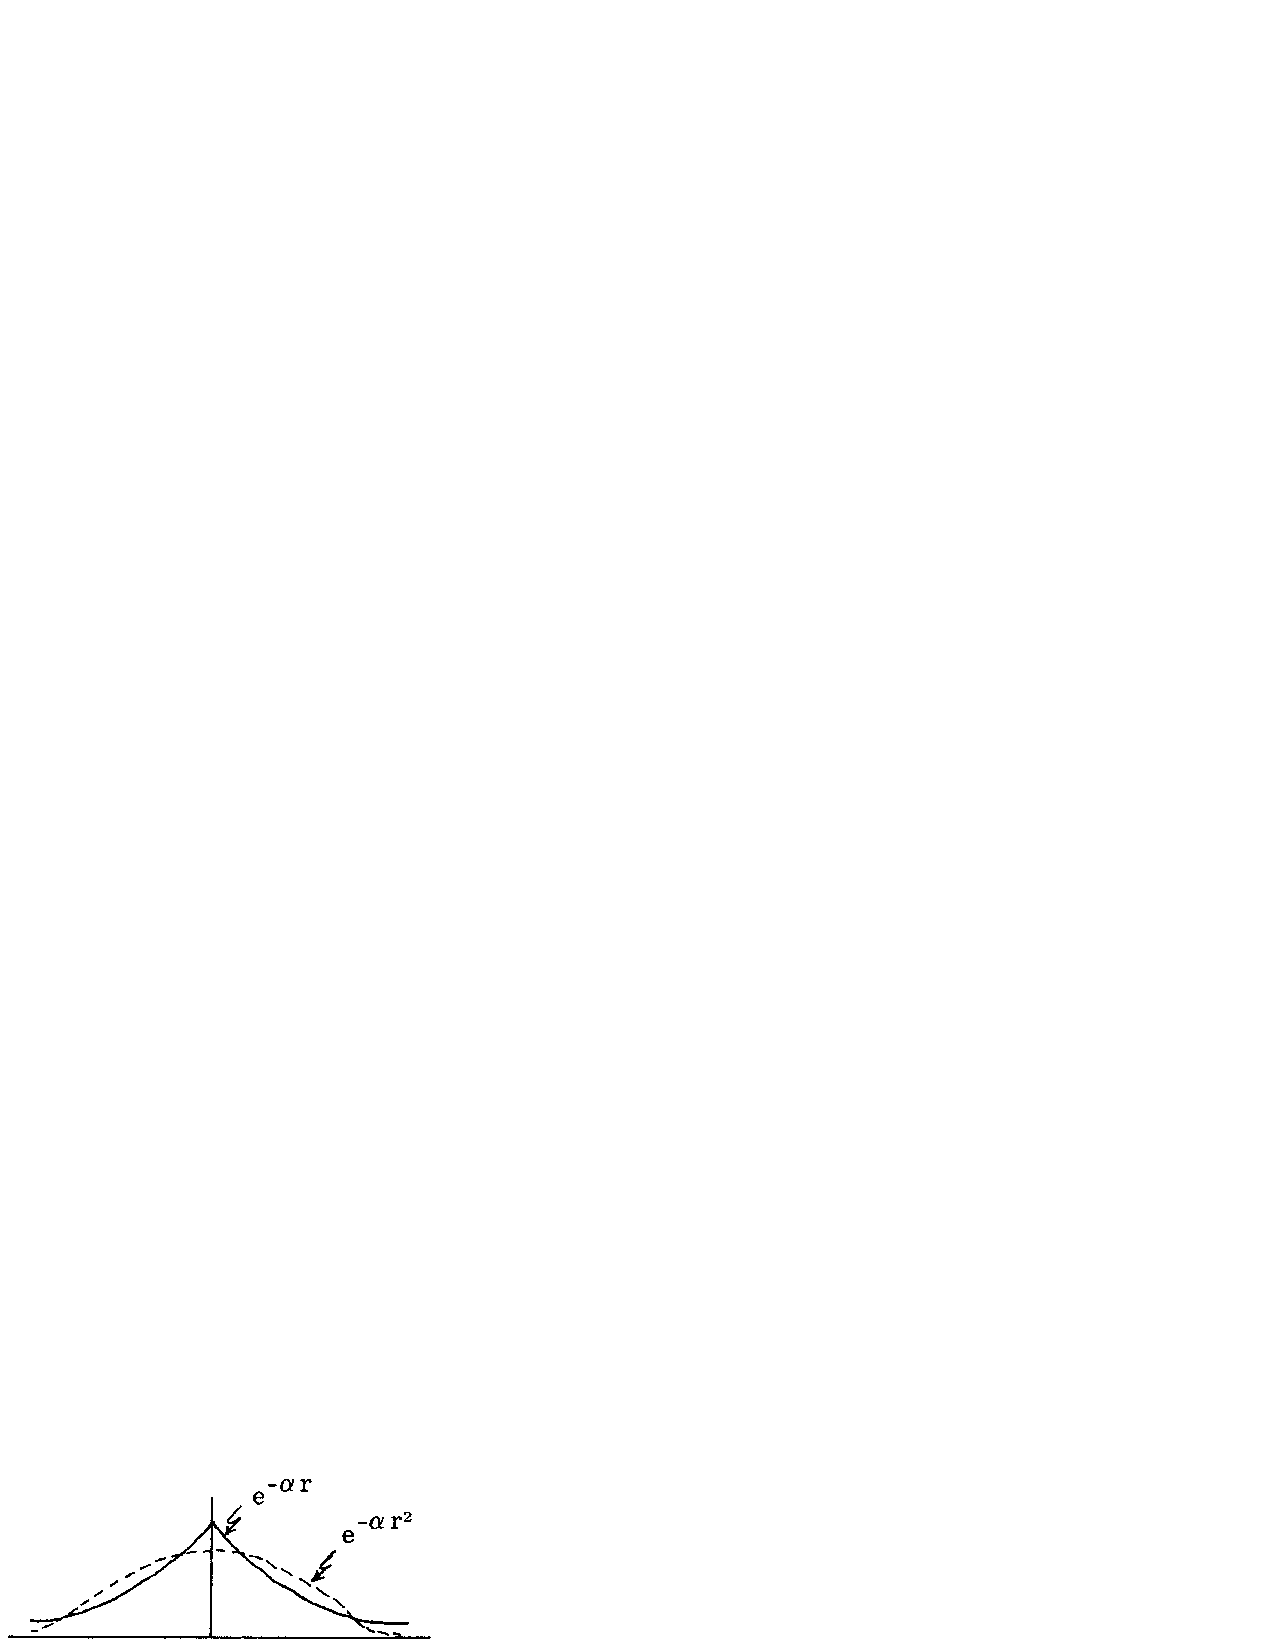
\includegraphics[scale=0.75]{fg15-1}
\caption{}
\label{chap15-fig1}
\end{figure}

As a result, it requires many Gaussian basis functions to describe the
character of an orbital near $r = 0$.  Thus, as shown in Appendix B, six
Gaussian functions are required to describe $H$ atom to $.00006 h$, and ten
Gaussians are required to describe the Hartree-Fock wavefunction of He to
$.00001 h$.  For Slater orbitals, two functions lead to better accuracy for He
atom.

Similarly, no single Gaussian function or finite linear combination of
them can describe the exponential long-range behavior
(\ref{chap15-eqno61}). This turns out to be a less serious problem
than the cusp condition. Optimizing the $\zeta$'s for Slater
functions, minimizing the energy, does not lead to $\zeta$'s
satisfying (\ref{chap15-eqno61}).  The important region energetically
is not $r
\rightarrow \infty$, but the region of 1 to 5 $a_0$ where the valence
electrons are concentrated.  To obtain a satisfactory description of
this region requires two functions with exponents appropriate for
describing this region, just as for Slater functions. Thus, the big
problem with Gaussian functions is the description of the core
character.

Tables \ref{chap15-tab7} and \ref{chap15-tab8} show the convergence of
the energy and other properties, for the ground state of oxygen atom,
as the number of Gaussian basis functions is increased. The density at
the nucleus, $\delta(O)$, is particularly poorly described, but other
properties are not too bad for the larger basis. The efficacy of
Gaussian and Slater bases is compared in Table \ref{chap15-tab9}.

The rate of convergence is only moderate, a $(7s3p)$ set being 
significantly better than the minimal set but worse than the marginal 
set $(3s2p)$.  Both the $(9s5p)$ and $(10s6p)$ Gaussian sets are better 
than the marginal set but not quite as good as the nominal, $(4s3p)$, 
set. The observed ratio of Gaussians to Slater is certainly less than 
three, 3. Because of the dependence of the number of two-electron 
integrals upon the fourth power of the number of basis functions, we 
thus must be able to compute integrals over Gaussians approximately 
$(3)^4 = 81$ times faster than over Slaters.  In fact, we are able to 
compute the integrals many times faster than this minimum requirement.

\begin{table}
\caption{Convergence of the energies of Hartree-Fock 
wavefunctions for the oxygen atom ($3p$) in a Gaussian basis.}
\label{chap15-tab7}
\begin{tabular}{ccccc}\\ \hline
Basis Set & $E_{HF}$ & $\epsilon(1s)$ & $\epsilon (2s)$ & $\epsilon 
(2p)$\cr

$(3s1p)$ & $-$71.2526 & $-$20.3867 & $-$1.2460 & $-$0.1988\cr
$(5s2p)$ & $-$74.2569 & $-$20.6892 & $-$1.1746 & $-$0.5007\cr
$(7s3p)$ & $-$74.7007 & $-$30.6447 & $-$1.2283 & $-$0.5974\cr
$(9s5p)$ & $-$74.8003 & $-$20.6663 & $-$1.2422 & $-$0.6294\cr
$(10s6p)$ & $-$74.8063 & $-$20.6680 & $-$1.2439 & $-$0.6512\cr
\hline
\end{tabular}
\end{table}

\begin{table}
\caption{Convergence of the radial integrals Hartree-Fock 
wavefunctions for the oxygen atom ($3p$) in a Gaussian basis.}
\label{chap15-tab8}
\begin{tabular}{cccccccc}\\ \hline
Basis Set&$\langle \delta (r) \rangle$&$\langle 1/r^3 
\rangle$&$\langle 1/r^2\rangle$&$\langle 1/r\rangle$&$\langle 
r\rangle$&$\langle r^2\rangle$& $\langle r^3\rangle$\cr

$(3s1p)$ & 172.8807 & 1.3654 & 220.3117 & 21.2111 & 7.4265 & 9.3770 & 
13.4559\cr
$(5s2p)$ & 260.0075 & 3.3252 & 251.4211 & 22.1208 & 7.3046 & 9.5586 & 
14.7764\cr
$(7s3p)$ & 281.8062 & 4.3243 & 255.4465 & 22.2464 & 7.4846 & 10.4702 & 
17.9645\cr
$(9s5p)$ & 295.8610 & 4.8708 & 256.7675 & 22.2581 & 7.5943 & 11.0640 & 
20.4697\cr
$(10s6p)$ & 301.3053 & 4.9094 & 257.0240 & 22.2584 & 7.6055 & 11.1372 & 
20.8549\cr
HF & 311.6681 & 4.9740 &  & 22.2601 &  & 11.1732\cr
\hline
\end{tabular}
\end{table}

\begin{table}
\caption{Comparison of the energies of Hartree-Fock 
wavefunctions for the first row atoms.}
\label{chap15-tab9}
\begin{tabular}{ccccccc}\\ \hline
Atom&\multicolumn{3}{c}{Gaussian}&\multicolumn{3}{c}{Slater}\cr
& $(7s3p)$ & $(9s5p)$ & $(10s6p)$ & $(2s1p)$ & $(3s2p)$ & $(4s3p)$\cr

Li & $-$7.4323 & $-$7.4325 & $-$7.4185 & $-$7.4323 & 
$-$7.4327\cr
Be & $-$ & $-$14.5721 & $-$14.5726 & $-$14.5567 & $-$14.5721 & 
$-$14.5730\cr
B & $-$24.5141 & $-$24.5271 & $-$24.5283 & $-$24.4984 & $-$24.5268 & 
$-$24.5290\cr
C & $-$37.6551 & $-$37.6852 & $-$37.6873 & $-$37.6224 & $-$37.6859 & 
$-$37.6885\cr
N & $-$54.3396 & $-$54.3953 & $-$54.3989 & $-$54.2689 & $-$54.3928 & 
$-$54.4008\cr
O & $-$74.7007 & $-$74.8003 & $-$74.8063 & $-$74.5404 & $-$74.7964 & 
$-$74.8091\cr
F & $-$99.2346 & $-$99.3956 & $-$99.4049 & $-$98.9421 & $-$99.3899 & 
$-$99.4089\cr
\hline
\end{tabular}
\end{table}

\subsubsection{Contraction of the Gaussian Basis Sets}

Even though the integrals over the large basis sets can be computed
quite efficiently, such sets also make the iterative solution of the matrix
Hartree-Fock equations very time consuming.  Numerous techniques have
been devised to accelerate the convergence of the solutions, thus reducing
the time requirement by reducing the number of iterations needed.  On the
other hand, a considerable savings in the time required per iteration would 
be affected if, in the large Gaussian sets, functions could be grouped 
together, i.e., contracted, and minipulated as only one function.  This 
procedure was first suggested by Whitten.$^8$  The contracted functions 
have the general form $\chi_i = \sum_{\rho} C {\bar{\chi}}_{\rho}$ 
where $\{{\bar{\chi}}_{\rho}\}$ denotes the original set of Gaussians, 
called the primitive basis set, and $\{ \chi_i \}$ the contracted 
set. The contraction coefficients, $\{ C_i\}$, are  input
data and, as we will show, can quite effectively be derived from just atomic
calculations.  If there are $Q$ functions in the primitive set and $P$ functions
in the contracted set, then contraction reduces the number of integrals to 
be manipulated by $(P/Q)^4$ and the iteration time by $(P \approx 
Q/2)^2$ or $(P \approx Q/2)^3$.  In practice, we shall see that little 
accuracy is lost if $(P \approx Q/2)$, so the contracted set will contain 
one-sixteenth the number of integrals and take one-fourth to 
one-eighth the time per iterations.

In going from atomic to molecular systems, the core orbitals are
relatively unchanged, e.g., $1s$ for first row atoms.  Because of
this, the linear combination of basis functions which describe the
inner shells can also be used in the molecule without undue loss of
accuracy.  A glance at the optimized exponents and coefficients of the
Gaussian basis functions for the $(9s5p)$ Hartree-Fock-Roothaan
wavefunction for the ground state of oxygen in Table
\ref{chap15-tab10}, reveals that many of the basis functions in both
the $s$-set and $p$-sets can be classified as inner shell type.  We do
not expect such primitive functions to extend beyond the atomic
regions of the molecule, so little should be lost upon contraction.

\begin{table}
\caption{The Hartree-Fock wavefunction for the ground 
state of the oxygen atom $(9s5p)$. Gaussian basis.$^a$}
\label{chap15-tab10}
\begin{tabular}{ccccccc}\\ \hline
Exponents &\multicolumn{3}{c}{Orbital Coefficients}\cr
& $1s$ & $2s$ & $2p$\cr

7816.5400 & 0.00118 & $-$0.00027\cr
1175.8200 & 0.00897 & $-$0.00207\cr
273.18800 & 0.04287 & $-$0.00979\cr
81.16960 & 0.14389 & $-$0.03574\cr
27.18360 & 0.35555 & $-$0.09508\cr
9.53223 & 0.46137 & $-$195.90\cr
3.42364 & 0.14017 & $-$0.03740\cr
0.93978 & $-$0.00058 & 0.59566\cr
0.28461 & 0.00139 & 0.52576\cr
35.18320 &  &  & 0.01541\cr
7.90403 &  &  & 0.09774\cr
2.30512 &  &  & 0.31066\cr
0.71706 &  &  & 0.49376\cr
0.21373 &  &  & 0.33604\cr
\hline
\end{tabular}\\
$^a$ See reference 10.
\end{table}

The best means of ascertaining the effects of contraction, is by a
series of calculations on a given molecule with various contracted
sets obtained from the same primitive set. For a given size contracted
set the mode of contraction can then be optimized. Such a study of the
water molecule has been carried out using a $(9s5p/4s)$ primitive
set.$^9$ The $(9s5p)$ oxygen set being taken from Huzinaga, Table
\ref{chap15-tab10}, and the $(4s)$ hydrogen set being obtained by
fitting four Gaussians to a Slater orbital with an exponent of 1.2.
The results of the calculations with the optimum $[3s2p/2s]$,
$[4s3p/2s]$, and $[5s3p/3s]$ sets are given in Table
\ref{chap15-tab11}.

\begin{table}
\caption{A comparison of the optimum contracted sets 
with the uncontracted $(9s5p/4s)$ set for the water molecules. Total energies,
orbital energies and dipole moment, in atomic units.}
\label{chap15-tab11}
\begin{tabular}{ccccc}\\ \hline

Property&\multicolumn{3}{c}{Contracted Sets}&Uncontracted Set\cr
& $[3s2p/2s]$ & $[4s3p/2s]$ & $[5s3p/3s]$ & $(9s5p/4s)$\cr

$E_{HF}$ & $-$76.0080 & $-$76.0104 & $-$76.0127 & $-$76.0132\cr
$\epsilon(1a_1)$ & $-$20.5547 & $-$20.5629 & $-$20.5608 & 
$-$20.5606\cr
$\epsilon(2a_1)$ & $-$1.3595 & $-$1.3609 & $-$1.3615 & $-$1.3609\cr
$\epsilon(1b_2)$ & $-$0.7147 & $-$0.7160 & $-$0.7159 & $-$0.7155\cr
$\epsilon(3a_1)$ & $-$0.5655 & $-$0.5670 & $-$0.5671 & $-$0.5673\cr
$\epsilon(1b_1)$ & $-$0.5037 & $-$0.5060 & $-$0.5059 & $-$0.5056\cr
$\mu$ & 1.0701 & 1.0519 & 1.0432 & 1.0428\cr
Number of Functions & 13 & 17 & 20 & 32\cr
\hline
\end{tabular}
\end{table}

Examining Table \ref{chap15-tab11} note that the energy is raised by
only 0.0052 atomic units, or 0.007 percent, by the loss in variational
freedom for the smallest basis set, $[3s2p/2s]$.  For the most
flexible contracted set investigated, the energy error is clearly
negligible; even this large a set has one-sixteenth the number of
integrals as does the primitive set. The $[4s3p/2s]$ set appears to be
a good compromise between accuracy and the desire to keep the basis
set as small as possible.  This selection is supported by calculations
on the nitrogen molecule where, because of the neighboring first row
atoms, the difference between the various contracted sets is much
larger, see Table \ref{chap15-tab12}.  Augmentation of this basis set
with suitable polarization functions should be far more important than
further flexibilization of the $(sp)$ set.  Note, for example, that
the contracted $[4s3p]$ Gaussian set for $N_2$ gives a lower energy
than the nominal $(4s3p)$ Slater set.  This, somewhat puzzling
observation, in view of the fact that $(9s5p)$ Gaussian set is far
inferior to a $(4s3p)$ Slater set for the atoms, is a reflection of
the optimum character of the Gaussian contracted set as well as the
energy to be gained from such flexibility in molecules.

While the actual contracted basis functions will not be given here,
we will comment that they can be easily rationalized on purely physical
grounds, and rules have been formulated to allow their extension to all of
the first row atoms. It is also important to note that the contraction 
coefficients were taken directly from the atomic calculations; this 
independence of the method from molecular information greatly enhances 
its generality.  The physical, rather than mathematical, nature of the 
contractions indicates that the optimum contracted sets should apply to 
other first row atoms and hydrogen in a wide variety of molecular 
environments. This conclusion is supported by calculations on a number 
of molecules not reported here.

\begin{table}
\caption{Calculations on the nitrogen molecule with 
Gaussian and Slater basis sets.  Gaussian primitive set is the $(9s5p)$ 
basis of Huzinaga.  All exponents are atom optimized.}
\label{chap15-tab12}
\begin{tabular}{ccccc}\\ \hline

Gaussian & $[3s2p]$ & $[4s2p]$ & $[4s3p]$ & $[5s3p]$\cr
$E_{HF}$ & $-$108.8153 & $-$108.8782 & $-$108.8877 & $-$108.8890\cr
Slater & $(4s2p)$ & $(4s3p)$ & $(5s3p)$\cr
$E_{HF}$ & $-$108.8617 & $-$108.8865 & $-$108.8967\cr
\hline
\end{tabular}
\end{table}

\subsubsection{Gaussian Lobe Functions}

The previous Gaussian calculations used Gaussians centered at the 
various nuclei and took each function to be factored into a radial part, a 
Gaussian, and an angular part, which was a spherical harmonic. The Gaussian
lobe method uses only spherically symmetric $1s$ Gaussians, 
$e^{-\alpha r^2}$; angular functions, such as a $p$-orbital, are 
approximated by linear combinations of $1s$-orbitals centered at the 
appropriate points in space. For example, a $2p_z$-orbital would be given by
\begin{equation}
~~~~~~~~~~~~~~~~~~~~ = \left[ e^{-\alpha(r-{\hat{Z}}_A)^2} - 
e^{-\alpha({\bar{r}}+{\hat{Z}}_A)^2}\right] {\hat{Z}}_A = Z_A 
{\bar{k}}
\end{equation}
Since a linear combination is, of course, not a pure $p$-function unless 
$Z_A \rightarrow 0$.  Thus, Hartree-Fock wavefunctions for atoms will not 
quite have the correct spatial symmetry.  This may affect some properties 
but not enough calculations have been reported, so a valid conclusion 
cannot be drawn.

Calculations with Gaussian lobe functions have been done on the first
row atoms by Whitten.$^8$ Whitten used a primitive $(10s5p)$ set, each
$p$ basis function being composed of two spherical Gaussians,
contracted to a $[3s1p]$ set and then optimized the exponents, and
displacements for the $p$-functions.  Unfortunately, Whitten chose a
rather poor contraction scheme for the $s$-orbitals, contraction for
the $p$-functions cannot affect the results as there is only one
$p$-atomic orbitals, resulting in a poor description of the
energetically important inner $s$-shell.  Whitten's description of the
valence region, on the other hand, seems to be as good as can be
obtained by Gaussians, as is illustrated in Table \ref{chap15-tab13}.
In Table \ref{chap15-tab14}, we compare the energies of the first row
atoms in a Gaussian lobe basis to those for conventional
Gaussians. Clearly, lobe functions are nearly as accurate as the
regular Gaussian orbitals.

The big advantage of this approach, Table \ref{chap15-tab14}, is the
simplicity with which the calculations can be done -- only the
formulas for $s$-orbitals need to be programmed!

\begin{table}
\caption{Comparison of the Gaussian lobe results for 
oxygen $(3p)$ with conventional Gaussian results. Radial integrals are 
in atomic units.}
\label{chap15-tab13}
\begin{tabular}{ccccc}\\ \hline
Basis Set & $\langle 1/r \rangle$ & $\langle ( 3 \cos^2 \Theta - 
1)/r^2\rangle$ & $\langle r^2\rangle$ & $\langle \delta (r)\rangle$\cr

$(9s5p)^a$ & 22.2581 & $-$1.9483 & 11.0640 & 295.86\cr
$(10s6p)^a$ & 22.2586 & $-$1.9643 & 11.1372 & 301.31\cr
$(10s5p)^b$ & 22.2548 & $-$1.9536 & 11.0518 & 288.60\cr
\hline
\end{tabular}\\
$^a$ Conventional.
$^b$ Lobes.
\end{table}

\begin{table}
\caption{The first row atoms in a Gaussian lobe basis 
and in conventional Gaussian basis.  Energy is in atomic units.}
\label{chap15-tab14}
\begin{tabular}{cccc}\\ \hline
Atom & Gaussian Lobe &\multicolumn{2}{c}{Conventional Gaussians}\cr &
$(10s5p)/[3s1p]$ & $(7s3p)$ & $(9s5p)$\cr

Li & $-$7.4312 &  & $-$7.4323\cr
Be & $-$14.5703 & $-$ & $-$14.5721\cr
B & $-$24.5241 & $-$24.5141 & $-$24.5271\cr
C & $-$37.6805 & $-$37.6551 & $-$37.6852\cr
N & $-$54.3882 & $-$3396 & $-$54.3953\cr
O & $-$74.7915 & $-$74.7007 & $-$71.8003\cr
F & $-$99.3823 & $-$99.2346 & $-$99.3956\cr
\hline
\end{tabular}
\end{table}

\section{Appendices}

\subsection{Molecular Integrals}

There are four basic types of integrals required in evaluating
\begin{equation}
\langle \chi_{\mu} \left| H^{HF} \right| \chi_{\nu} \rangle
\label{chap15app-eqno1}
\end{equation}
and indeed the energy of any other type of wavefunction.  They are as follows
\begin{tabular}{ccc}\\
Integral & Name & Number of Electrons\cr
$\langle \chi_{\mu} | \chi_{\nu} \rangle$ & overlap & one\cr
$\langle \chi_{\nu} \left| - {1 \over 2} \nabla^2 \right| 
\chi_{\mu}\rangle$ & kinetic energy & one\cr
$\langle \chi_{\mu} \left| {Z_A \over r_A} \right| 
\chi_{\nu}\rangle$ & nuclear attraction & one\cr
$\langle \chi_{\mu} \chi_{\nu} \left| {1 \over r_{12}} \right| 
\chi_{\sigma} \chi_{\rho} \rangle$ & electron repulsion & two\cr
\end{tabular}
If there are $P$ basis functions and $Z$ nuclei, there will be $P(P + 1)/2$ 
overlap and kinetic energy integrals, $ZP(P + 1) /2$ nuclear attraction 
integration, and $1/8(P^4 + 2P^3 + 4P^2 + 2P)$ two-electron 
integrals.  To obtain these figures, only the interchange symmetry of 
the integrals have been taken into account; in fact, that by spatial 
symmetry some integrals are equal and some are zero, has been neglected. 
This dependence of the number of two-electron integrals upon the fourth 
power of the number of basis functions requires that we use efficient 
methods to calculate the integrals over the basis function. For many
years this was the major bottleneck in carrying out molecular calculations.

\subsubsection{Slater Orbitals}

If the Slater basis functions are centered on the various nuclei which
make up the framework of the molecule, then the integrals which arise
in evaluating (\ref{chap15app-eqno1}) are conveniently classified
according to the number of different centers involved. For example,
overlap and kinetic energy integrals can, at most, involve two
centers, nuclear attraction integrals three centers and two-electron
integrals four centers.  As we shall see, the main problem in
computing these integrals is finding a common ground over which to
carry out the indicated integrations, i.e., in finding a convenient
coordinate system in terms of which all the functions in the integrand
are easily expressible.

Only one center integrals occur in atomic calculations and none of the
integrals of this type are very difficult.  For this reason we shall not 
discuss one-center integrals explicitly.  About the only point worth 
noting is that the expansion$^{11}$ of $1/r_{12}$
\begin{equation}
{1 \over r_{12}} = \sum^{\infty}_{l=0} {r^l_< \over r^{l+1}_>} 
\sum^{l}_{m=-l} {(l-m)! \over (l+m)!} P^m_l \left( \cos \Theta_1 
\right) P^m_l \left( \cos \Theta_2 \right) e^{2m(\varphi_1-\varphi_2)}
\end{equation}
is needed for evaluating the two-electron integrals.

Two center integrals first occur in diatomic molecules, and it is here
that hints of the problems which will occur for polyatomic systems are first
found. For example, the two-electron exchange integral
\begin{equation}
\int \int \chi_{A \nu} (1) \chi_{B \mu} {1 \over r_{12}} \chi_{A 
\sigma} (2) \chi_{B \rho} (2) dv_1 dv_2
\end{equation}
does not have a closed form solution.  In this integral, the first subscript
represents the center, the second represents the function.  Fortunately, all 
of the other types of two-center integrals do have closed form solutions.

\subsubsection{A Two-Center Integral}

As an example of the problems and techniques which arise in connection
with two-center integrals, we will consider a rather simple example, the 
two-center nuclear attraction integral
\begin{equation}
v \left( 1s_A, 1s_B , {-1 \over r_B}\right) = \int 1s_A {1 \over r_B} 
1s_B d \tau = \langle 1s_A \left| {1 \over r_B} \right| 1s_B \rangle
\end{equation}
using the coordinate system
\vskip 1.25truein
\noindent
Note that there are two different $\Theta$'s but only one $\varphi$.  The 
integral to be done is		
\begin{equation}
\langle 1s_A \left| {1 \over r_B} \right| 1s_B \rangle = 
\left( {\zeta_A \zeta_B \over \pi^2} \right)^{{1 \over 2}} \int e^{-\zeta_A 
r_A} {1 \over r_B} e^{-\zeta_Br_B} d \tau
\label{chap15app-eqno2}
\end{equation}
from the law of cosines, we see that
\begin{equation}
r_B = \sqrt{r^2_A + R^2 - 2r_AR \cos \Theta_a}
\end{equation}
Since $r_B$, by definition, is a positive quantity, we must always take the 
positive sign of the square root, which will give rise to certain 
complications.  Using this expression for $r_B$, the integral becomes
\begin{equation}
\langle 1s_A \left| {1 \over r_B} \right| 1s_B \rangle = 
\left( {\zeta_A \zeta_B \over \pi^2} \right)^{{1 \over 2}} 
\int\limits_{0}^{\infty} \int\limits_{0}^{\pi} \int\limits^{2 \pi}_{0} 
{e^{-\zeta_Ar_A} e^{-\zeta_B\sqrt{r^2_A+R^2-2r_AR\cos \Theta_A}} 
\over \sqrt{r^2_A+R^2 -2r_AR \cos \Theta_A}} \times r^2_A \sin 
\Theta_A dr_A d \Theta_A d \varphi
\end{equation}
Since the integrand does not depend on $\varphi$, this variable can 
be integrated immediately to give $2\pi$. The integral over 
$d\Theta_A$ can be done by making the substitutions
$r^2_A + R^2 - 2r_A R \cos \Theta_A = a + bx = y$ and $y = z^2$.  
Doing this, we find that
\begin{equation}
\langle 1s_A \left| {1 \over r_B} \right| 1s_B \rangle = {2 \over R} 
\sqrt{\zeta^3_A \zeta_B} \int\limits^{\infty}_{0} e^{-\zeta_Ar_A} 
\left[ {e^{-\zeta|r_A-R|} - e^{-\zeta_B(r_A + R)} \over r_A} \right] 
r^2_A dr_A
\end{equation}
Note we have had to use $| r_A - R|$ rather than just $(r_A - R)$. This
arises from the positive nature of $r_B$ mentioned previously.  To 
keep $| r_A - R|$ positive, we can break up the integral over $r_A$ 
into two parts.  First an integral from 0 to $R$, the interval in which 
$r_A \leq R$, and second, an integral from $R$ to $\infty$,
the interval in which $r_A \geq R$.  The resulting radial integrals can be
integrated by parts to yield the final result
\begin{eqnarray}
\langle 1s_A \left| {1 \over r_B} \right| 1s_B \rangle & =& {2 \over 
R} \sqrt{\zeta^3_A\zeta_B} \left\{e^{-\zeta_BR} \left[ {4 \over 
(\zeta_B-\zeta_A)^2} - {1 \over (\zeta_B+\zeta_A)^2} \right]\right.\cr
&& \left. + e^{-\zeta_AR} \left[ {R \over \zeta_B-\zeta_A}+{R \over 
\zeta_B+\zeta_A} - {1 \over (\zeta_B-\zeta_A)^2} + {1 \over 
(\zeta_B+\zeta_A)^2}\right] \right\}
\end{eqnarray}
Note this formula does not apply if $\zeta_A = \zeta_B$ and, 
in fact, difficulties will arise if $\zeta_B \approx \zeta_A$.  For 
these cases, a separate formula should be derived or L'Hospital's Rule 
applied to the above to obtain the proper limiting form.

The above integral can also be done to prolate spheroidal coordinates
$\xi , \eta)$ defined by
\begin{equation}
\xi = {r_A+r_B \over R}
\end{equation}
and
\begin{equation}
\eta = {r_A - r_B \over r}
\end{equation}
This separates the variables, reducing the original three-dimensional 
integral to a product of one-dimensional integrations.  However, we will 
not pursue the topic further.

\subsubsection{Zeta Function Expansions}

It is with three and four center integrals that severe computational
difficulties arise. Whereas for just two centers all of the integrals except
the two-electron exchange can be solved in closed form, none of the three
and four center integrals can be so simplified.  One means of reducing the
problem to computational form is by the introduction of a zeta 
function,$^{12}$ $\zeta_{m,n}(\beta , r_A , R)$, defined by
\begin{equation}
r^{m-1}_B e^{-\alpha_Br_B} = \sum^{\infty}_{n=0} {(2n+1) \over 
\sqrt{r}_AR} P_n \left( \cos \Theta_A \right) \zeta_{m,n} ( \alpha_B, 
r_A; R)
\end{equation}
with the coordinate system identical to that used previously to compute
\begin{equation}
\langle 1s_A \left| {1 \over r_B} \right| 1s_B \rangle
\end{equation}
Thus, the zeta function expansion is used to expand the radial portion of
a Slater orbital from one center ($B$) onto another ($A$).  The transformation
of the angular portion is trivial.  The detailed form of the zeta function is
rather complicated and we shall not delve into it any further here.  We shall
merely note that for $m = 0$ the zeta functions can be expressed as products
of Bessel functions of imaginary argument and half-odd integral order, and
that the zeta functions of higher $m$ can be computed by means of simple
recurrence formulas.

Some of the general properties of the zeta function expansion can be
obtained without a knowledge of their exact radial form, however. Let
us consider the two-center potential energy integral calculated
previously (\ref{chap15app-eqno2}).  The zeta function expansion can
be used to expand $e^{\zeta_Ar_A}$ onto center $B$, the integral
becoming
\begin{eqnarray}
\langle 1s_A \left| {1 \over r_B} \right| 1s_B \rangle & = & \left( 
{\zeta_A \zeta_B \over \pi^2} \right)^{{1 \over 2}} \sum_{n} {(2n+1) 
\over \sqrt{R}} \int\limits^{\infty}_{0} {\zeta_{1,n}(\zeta_A,r_B;R) 
\over \sqrt{r}_B} {e^{-\zeta_Br_B} \over r_B}\cr
&& \times r^2_B dr_B \int\limits^{\pi}_{- \pi} P_n ( \cos \Theta_B ) 
\sin \Theta_B d \Theta_B \int\limits^{2\pi}_{0} d \varphi
\end{eqnarray}
The $\varphi$-integral gives $2\pi$.  The orthogonality property of 
the Legendre functions eliminates all but the $n = 0$ term of the series, i.e.,
\begin{equation}
\int\limits^{\pi}_{-\pi} P_n ( \cos \Theta_B ) \sin \Theta_B d 
\Theta_B = 2 \delta_{\eta o}
\end{equation}
So,
\begin{equation}
\langle 1s_A \left| {1 \over r_B} \right| 1s_B \rangle = 4 
\left( {\zeta^3_A \zeta^3_B \over R} \right)^{{1 \over 2}} 
\int\limits^{\infty}_{0} r^{{1 \over 2}}_B \zeta_{1,0} (\zeta_A, 
r_B;R) e^{-\zeta_B r_B} dr_B
\end{equation}
Thus, only one term in the finite series expansion of 
$e^{-\alpha_Ar_A}$ contributes!  This, of course, just reflects the 
fact that a closed form solution exists for
this integral.  To see what happens in a more general case, let us consider
the three-center, one-electron nuclear attraction integral
\begin{equation}
\langle 1s_A \left| {1 \over r_B} \right| 1s_C \rangle = 
\left( {\zeta^3_A \zeta^3_C \over \pi^2} \right)^{{1 \over 2}} 
\int e^{- \zeta_Ar_A} {1 \over r_B} e^{- \zeta_Cr_C} d \tau
\end{equation}
The zeta function can be used to expand $e^{-\zeta_Cr_C}$ onto 
center $A$. In a similar manner, $1/r_B$ can be expanded onto $A$. The 
integral will now be a sum of two infinite series
\begin{eqnarray}
\langle 1s_A \left| {1 \over r_B} \right| 1s_C \rangle & = &
\left( {\zeta^3_A \zeta^3_C \over \pi^2} \right)^{{1 \over 2}} 
\sum_{l} \sum_{l^{\prime}} \int\limits^{\infty}_{0} 
\int\limits^{\pi}_{0} \int\limits^{2 \pi}_{0} e^{-\zeta_Ar_A} 
\left[ {r^l_< \over r^{l+1}_>} P_l ( \cos \Theta_{AB}) \right]\cr
&& \times \left[ {(2l^{\prime}+1) \over \sqrt{r_AR}} 
\zeta_{1,l^{\prime}} ( \zeta_C , r_A; R_{AC}) P_{l^{\prime}} ( \cos 
\Theta_{AC})\right] r^2_A \sin \Theta_A dr_A d \Theta_A d \varphi_A
\end{eqnarray}
with the angles $\Theta_{AB}$ and $\Theta_{AC}$ defined as
\vskip 1.25truein
\noindent
By an extension of the orthogonality relations between the Legendre 
functions, it can be shown that
\begin{equation}
\int\limits^{\pi}_{-\pi} P_l ( \cos \Theta_{AB}) P_{l^{\prime}} ( \cos 
\Theta_{AC} ) \sin \Theta_A d \Theta_A = {2 \over 2l+1} P_l ( \cos 
\Theta) \delta_{ll^{\prime}}
\end{equation}
$\Theta$ was defined earlier.  Finally then, the integral becomes
\begin{equation}
\langle 1s_A \left| {1 \over r_C} \right| 1s_B \rangle = 
\left( {\zeta^3_A \zeta^3_B \over \pi^2} \right)^{{1 \over 2}} 
\sum_{l} {4 \pi \over 2l+1} P_l ( \cos \Theta ) 
\int\limits^{\infty}_{0} {r^l \over r^{l+1}} r^{{3 \over 2}}_{A} 
e^{-\zeta_ar_A} \zeta_{1,l} ( \zeta_C , r_A; R_{AC} ) \times dr_A
\end{equation}

There is no truncation here, we must sum an infinite series!  The relevant
question now is, how fast does the series converge Experience has shown
that it usually requires less than thirty terms although in some cases many
more may be required.  It is the calculation of all of these terms in the 
series which accounts for large computing times. In a similar manner, it can 
be shown that for four-center, two-electron integrals a doubly infinite series 
must be summed. It has been estimated that over 70 percent of the time required
for calculations on polyatomic molecules is spent evaluating three-center,
one-electron, and three-center and four-center two-electron integrals.

\subsubsection{The Gaussian Transform Approach}

Another approach to the multi-center integral problem is by means of
the Gaussian Transform Method.$^{13,14}$  This method makes use of the integral
transform
\begin{equation}
e^{-\zeta r_A} = {\zeta \over 2 \sqrt{\pi}} \int\limits^{\infty}_{0} 
s^{-{3 \over 2}} e^{-sr^2_A} ds
\end{equation}
To see how the Gaussian transform method is used, let us turn once again
to our favorite integral, the nuclear attraction integral
\begin{equation}
\langle 1s_A \left| {1 \over r_B} \right| 1s_B \rangle = 
\left( {\zeta_A \zeta_B \over \pi^2} \right)^{{1 \over 2}} 
\int\limits_{\pi} e^{-\zeta_Ar_A} {1 \over r_B} e^{-\zeta_B r_B} d \tau
\end{equation} 
Using the Gaussian transform for $e^{-\zeta_Ar_A}$ and $e^{-\zeta_B 
r_B}$ we obtain
\begin{eqnarray}
\langle 1s_A \left| {1 \over r_B} \right| 1s_B \rangle & = &
\left( {\zeta^3_A \zeta^3_B \over R} \right)^{{1 \over 2}} 
\left( {\zeta^3_A \zeta^3_B \over \pi^2} \right) 
\left( {\zeta_B \over 2 \sqrt{\pi}} \right)
\left( {\zeta_B \over 2 \sqrt{\pi}} \right)\cr
&& \times \int\limits_{\tau} d \tau {1 \over r_B} \int\limits^{\infty}_{0} 
ds_A s_A^{-{3 \over 2}} e^{-{\zeta^2_A \over 4s_A}} e^{-s_Ar^2_A}
\int\limits^{\infty}_{0} ds_Bs_B^{-{3 \over 2}} e^{-{\zeta^2_B \over 
4s_B}} e^{-s_Br_B^2}
\end{eqnarray}
or
\begin{eqnarray}
\langle 1s_A \left| {1 \over r_B} \right| 1s_B \rangle & = & {1 \over 4} 
\left( {\zeta^5_A \zeta^5_B \over \pi^4} \right)^{{1 \over 2}} 
\int\limits^{\infty}_{0} ds_As_A^{-{3 \over 2}} e^{-{\zeta^2_A \over 
rs_A}}\cr 
&& \times \int\limits^{\infty}_{0} ds_B s_B^{-{3 \over 2}} 
e^{-{\zeta^2_B \over 4s_B}} \langle 1s_A \left| {1 \over r_B} \right| 
1s_B \rangle_g
\end{eqnarray}
where
\begin{equation}
\langle 1s_B \left| {1 \over r_B} \right| 1s_B \rangle_g = 
\int\limits_{\tau} e^{-s_Ar_A^2} {1 \over r_B} e^{-s_Br_B^2} d \tau
\end{equation}
is the corresponding nuclear attraction integral over unnormalized 
Gaussians. We will not discuss the Gaussian integral at present, it will be 
treated in more detail in the next section. The only fact that is of 
interest here is that this integral can be obtained in closed form. As 
we can see, the utility of this method will depend on the efficiency 
with which the integrals over the transformation coordinates, $S_A$ 
and $S_B$, can be performed.  One of the integrations can be done 
analytically by an appropriate change of variables.  Actually, this 
simplification can be accomplished by either of two 
transformations.  The first, which is the usual procedure, results 
in finite range numerical integrations over a well-behaved integral 
which can be expressed as an infinite series of hyperbolic Bessel 
function. The second, called the alternate transform method, replaces 
two of the integrations with an integral over an infinite range of a 
spherical Bessel function which oscillates in sign.  At first, it was 
felt that this oscillatory character would lead to problems of
instability in the resulting numerical integration.  However, R. M. Stevens,
Harvard, has studied these complications and has found that the resulting
errors are inconsequential. At present, it appears that the alternate 
transform method is the most efficient means of calculating integrals 
over Slater orbitals for polyatomic systems.

So far, for the Gaussian transform method we have considered integrals
only over $1s$ orbitals. While in the zeta function expansion the 
generalization to higher orbitals was obvious, in the Gaussian transform 
method, use is made of a differential operator technique.  Note, for 
example, that
\begin{equation}
2s = re^{-\alpha r} = - {\partial \over \partial \alpha} e^{-\alpha 
r} = - {\partial \over \partial \alpha} (1s)
\end{equation}
neglecting normalization.  These operators are then applied directly to the
formulas derived in terms of $1s$ orbitals, interchanging in the order of 
integration and differentiation when necessary.

\subsubsection{Programs}

Before closing the topic of integrals over Slater orbitals, we should 
mention something about the application of these techniques. Programs based
on the zeta function expansion were written by R. M. Pitzer, D. Ellis, W.
E. Palke, and other, the resulting integrals package being called the 
Cambridge Programs. I. Shavitt developed the Gaussian transfrom method and
wrote an integral package based on this method. R. M. Stevens, as 
mentioned earlier, investigated the alternate transform method and has written
the corresponding integrals package. To give some idea of the 
comparative speed of these methods, below we list approximate integral 
computation times for the ethane molecules in a minimum basis set: zeta 
function $\sim$90 minutes; Gaussian transform $\sim$90 minutes; and, the 
alternate transform, $\sim$6 minutes.  We see that the zeta function and 
Gaussian transform methods are nearly comparable but that the alternate 
transform method is more than an order of magnitude faster.

\subsection{Gaussian-Type Orbitals}

Another approach to the problem of matrix Hartree-Fock calculations
on polyatomic molecules is just to forget about Slater orbitals entirely 
and use basis sets containing only Gaussian orbitals. As we shall see in this 
section, the principle advantage of Gaussians is that all of the integrals 
required for such calculations can be obtained in closed form, their major 
disadvantage being the relatively slow convergence of the expansion. The 
problems arising from the correspondingly larger basis sets can be 
overcome, however, and the use of Gaussian-type basis functions provides 
the most efficient means  of obtaining moderately accurate wavefunctions 
for polyatomic systems.

The property of Gaussians directly responsible for the ease with which
multi-center integrals can be computed, is that the product of two 
Gaussians located at arbitrary points is another Gaussian situated along the 
line centers, i.e.,
\begin{equation}
e^{-\alpha_A r^2_A} e^{-\alpha_Br^2_B} = \exp \left\{ - {\alpha_A 
\alpha_B \over \alpha_A + \alpha_B} {\bar{A}} {\bar{B}}^2 \right\} 
e^{-(\alpha_A+\alpha_B)r^2_Q}
\label{chap15app-eqno3}
\end{equation}
The coordinates of the point $Q$ being given by
\begin{equation}
Q_x = {\alpha_AA_x + \alpha_BB_x \over \alpha_A + \alpha_B},
\end{equation}
etc.  ${\bar{A}}{\bar{B}}$ is the distance between centers $A$ and $B$ 
located at ($A_x , A_y, A_z$) and ($B_x , B_y, B_z$) in the master 
coordinate system.

\subsection{Calculation of the Integrals}

As in the previous section, we shall first take a look at the calculation
of molecular integrals.  To illustrate the techniques that have been 
developed for calculating integrals over Gaussian orbitals, we will work 
out the  nuclear attraction integral encountered in our discussion of the 
Gaussian transform method
\begin{equation}
\langle 1s_A \left| {1 \over r_B} \right| 1s_B \rangle = N(s_A)N(s_B) 
\int e^{-\alpha_Ar^2_A} {1 \over r_B} e^{-\alpha_Br^2_B} d \tau
\label{chap15app-eqno4}
\end{equation}

In evaluating this integral, we will make use of another useful
property of Gaussian functions, namely that inverse powers of $r$ can
be expressed as integrals over Gaussian functions. For
(\ref{chap15app-eqno4}), we see
\begin{equation}
{1 \over r} = {1 \over \sqrt{\pi}} \int\limits^{\infty}_{0} dss^{-{1 
\over 2}} e^{-sr^2}
\label{chap15app-eqno5}
\end{equation}
Using (\ref{chap15app-eqno3}) and (\ref{chap15app-eqno5}), making use
of these special properties of Gaussians, the nuclear attraction
integral (\ref{chap15app-eqno4}) becomes
\begin{equation}
\langle 1s_A \left| {1 \over r_B} \right| 1s_B \rangle_g = {2N_AN_B 
\over \sqrt{\pi}} \exp \left\{ - {\alpha_A \alpha_B \over \alpha_A + 
\alpha_B} {\bar{A}} {\bar{B}}^2\right\} \int\limits^{\infty}_{0} 
dss^{-{1 \over 2}} \int\limits_{\tau} e^{-(\alpha_A+ \alpha_B)r^2_Q} 
e^{-sr^2_B} d \tau
\end{equation}
Again we can make use of the special multiplication properties of Gaussians
and the fact that the exponential functions are separable in ($x, y, z$) to 
yield
\begin{eqnarray}
\langle 1s_A \left| {1 \over r_B} \right| 1s_B \rangle_g & = &
{2N_AN_B \over \sqrt{\pi}} \exp \left\{ - {\alpha_A \alpha_B \over \alpha_A + 
\alpha_B} {\bar{A}} {\bar{B}}^2\right\} \int\limits^{\infty}_{0} 
dss^{-{1 \over 2}} \exp \left\{ - {\alpha_A \alpha_B \over \alpha_A + 
\alpha_B} {\bar{B}} {\bar{Q}}^2\right\}\cr
&& \times \int\limits^{\infty}_{- \infty} dx_p 
e^{-(\alpha_A+\alpha_B+s)x^2_p} \int\limits^{\infty}_{-\infty} dy_p 
e^{-(\alpha_A+\alpha_B+s)y^2_p} \int\limits^{\infty}_{-\infty} dz_p 
e^{-(\alpha_A+\alpha_B+s)z^2_p}
\end{eqnarray}
The integrals over the spatial coordinates, $x_p=x-p_x$, etc., are of standard
form
\begin{equation}
\int\limits^{\infty}_{-\infty} e^{-\alpha x^2} dx = \sqrt{{\pi \over r}}
\end{equation}
Thus, the integral becomes
\begin{eqnarray}
\langle 1s_A \left| {1 \over r_B} \right| 1s_B \rangle_g & = &2 \pi 
N_AN_B \exp \left\{ - {\alpha_A \alpha_B \over \alpha_A + 
\alpha_B} {\bar{A}} {\bar{B}}^2\right\}\cr
&& \times \int\limits^{\infty}_{0} dss^{{1 \over 2}} \exp \left\{ 
{\alpha_A \alpha_B \over \alpha_A + 
\alpha_B +s} {\bar{B}} {\bar{Q}}^2\right\} \left( \alpha_A + \alpha_B + 
s \right)^{{1 \over 2}}
\end{eqnarray}
The integral over the transformation vaxiable, $S$, can be put into a standard
form with the following change of variables
\begin{equation}
{1 \over 1 - t^2} = {\alpha_A + \alpha_B + S \over \alpha_A + \alpha_B}
\end{equation}
or
\begin{equation}
s = ( \alpha_A + \alpha_B ) {t^2 \over 1 - t^2}
\end{equation}
and
\begin{equation}
ds = 1 ( \alpha_A + \alpha_B ) {tdt \over (1-t^2)^2}
\end{equation}
yielding
\begin{equation}
\langle 1s_A \left| {1 \over r_B} \right| 1s_B \rangle_g = 
{4 \pi N_AN_B \over \alpha_A + \alpha_B} \exp \left\{ - {-\alpha_A 
\alpha_B \over \alpha_A + \alpha_B} {\bar{A}} {\bar{B}}^2 \right\}
\int\limits^{1}_{0} e^{-(\alpha_A + \alpha_B) {\bar{B}}{\bar{Q}}^2t^2} dt
\end{equation}
Let us now define the class of functions
\begin{equation}
f_m (u) = \int\limits^{1}_{0} t^{2m} e^{-ut^2} dt
\end{equation}
which are a generalized form of the incomplete gamma function. This 
function will occur whenever a LaPlace transform is used to remove inverse 
powers of $r$ or $r_{12}$ from the integrand.  It can be evaluated using 
polynomial approximation or interpolation. Finally then, the integral becomes
\begin{equation}
\langle 1s_A \left| {1 \over r_B} \right| 1s_B \rangle = 
{4 \pi N_AN_B \over \alpha_A + \alpha_B} \exp 
\left\{ - {-\alpha_A \alpha_B \over \alpha_A + \alpha_B} 
{\bar{A}} {\bar{B}}^2 \right\} F_0 \left[ \left( \alpha_A + \alpha_B 
\right) {\bar{B}} {\bar{Q}}^2 \right]
\end{equation}

Looking back over our derivation, we note that the number of centers
involved was immaterial. Thus, the general nuclear attraction integral over
$1s$ orbitals can be written as
\begin{equation}
\langle 1s_A \left| {1 \over r_B} \right| 1s_C \rangle = 
{4 \pi N_AN_B \over \alpha_A + \alpha_C} \exp \left\{ - {-\alpha_A 
\alpha_C \over \alpha_A + \alpha_C} {\bar{A}} {\bar{C}}^2 \right\} 
F_0 \left[ \left( \alpha_A + \alpha_C \right) {\bar{B}} {\bar{Q}}^2 
\right]
\end{equation}
A closed form solution exists even for three-center integrals!

In a similar manner, we can show that the four-center, two-electron
integral,
\begin{equation}
\langle 1s_a 1s_b \left| {1 \over r_{12}} \right| 1s_c 1s_d \rangle ,
\end{equation}
first reduced to a two-center, two-electron Coulomb integral,
\begin{equation}
\langle 1s_p \left| {1 \over r_{12}} \right| 1s_q \rangle .
\end{equation}
and then use of the LaPlace transform for $1/r_{12}$ reduced the integral to
a closed form solution.  Thus, we see that all of the energy integrals over
Gaussian basis functions can be put into closed form. It is also easy to 
show that nearly all integrals which arise in regard to molecular systems, 
e.g., for one-electron and two-electron properties, correlation factors, etc., 
can be evaluated in closed form.

Integrals over higher orbitals can be derived by differential operator
techniques, as in the Gaussian transform method, or by explicit calculation
over the orbitals themselves.

\subsection{Huzinaga's Tables}

Various tables from Huzinaga,$^{10}$ are given below. Table
\ref{chap15b-tab1} shows how well various numbers of $1s$ Gaussian or
$2p$ Gaussians can describe a $1s$ Slater or $2p$ Slater function,
respectively. Table \ref{chap15b-tab2} gives the expansion
coefficients of a $1s$ Slater orbital in terms of $1s$
Gaussians. Thus,
\begin{equation}
\chi = 0.274e^{-1.332r^2} + 0.821e^{-0.202r^2}
\end{equation}
provides the best description of
\begin{equation}
{1 \over \sqrt{\pi}} e^{-r}
\end{equation}
if two Gaussians are to be used.  If one wants to describe a scaled Slater
orbital
\begin{equation}
\sqrt{{\zeta^3 \over \pi}} e^{-\zeta r}
\end{equation}
then the exponents ($\alpha_r$) of Table \ref{chap15b-tab2} must be
replaced by ${\bar{\alpha}}_r = \zeta^2 \alpha_r$, for $2p$ the
relation is ${\bar{\alpha}}_r = (2 \zeta)^2\alpha_r$. Table
\ref{chap15b-tab3} shows the corresponding relationships for $2p$
orbitals.

\begin{table}
\caption{$\langle Z^{-1}H_s\rangle$ in atomic units. $1s$, 
exact value = $-$0.5, and for $2p$, exact value = $-$0.125,
Slater-type orbitals.  $N$ is the number of terms in the Gaussian-type
orbital expansion.}
\label{chap15b-tab1}
\begin{tabular}{ccccc}\\ \hline
$N$ &\multicolumn{2}{c}{$(1s)_s-(1s)_g$}&
\multicolumn{2}{c}{$(2p)_s-(2p)_g$}\cr
&Present Calculation& Singer & Present Calculation& Reaves\cr

1 & $-$0.424413 &  & $-$0.113177 & $-$0.1113177\cr
2 & $-$0.485813 & $-$0.486 & $-$0.123289 & $-$0.123289\cr
3 & $-$0.496979 & $-$0.49689 & $-$0.124728 & $-$0.124728\cr
4 & $-$0.499277 & $-$0.49928 & $-$0.124952 & $-$0.124952\cr
5 & $-$0.499809 & $-$0.49976 & $-$0.124991\cr
6 & $-$0.499940 & $-$0.49988 & $-$0.124998\cr
7 & $-$0.499976\cr
8 & $-$0.499991 & $-$0.49992\cr
9 & $-$0.499997\cr
10 & $-$0.499999\cr
\hline
\end{tabular}
\end{table}

\begin{table}
\caption{Parameters of Gaussian-type orbital expansions, $(1s)_s - (1s)_g$.}
\label{chap15b-tab2}
\begin{tabular}{ccc}\\ \hline
$B$ & $\alpha_i$ & $C_i$\cr

2 & 0.201527 & 0.82123\cr
 & 1.33248 & 0.27441\cr
3 & 0.151374 & 0.64767\cr
 & 0.681277 & 0.40789\cr
 & 4.50038 & 0.07048\cr
4 & 0.123317 & 0.50907\cr
 & 0.453757 & 0.47449\cr
 & 2.01330 & 0.13424\cr
 & 13.3615 & 0.01906\cr
5 & 0.101309 & 0.37602\cr
 & 0.321144 & 0.50822\cr
 & 1.14680 & 0.20572\cr
 & 5.05796 & 0.04575\cr
 & 33.6444 & 0.00612\cr
6 & 0.082217 & 0.24260\cr 
 & 0.224660 & 0.49221\cr
 & 0.673320 & 0.29430\cr
 & 2.34648 & 0.09280\cr
 & 10.2465 & 0.01938\cr
 & 68.1600 & 0.00255\cr
7 & 0.060738 & 0.11220\cr
 & 0.155858 & 0.44842\cr
 & 0.43661 & 0.38487\cr
 & 1.370498 & 0.15161\cr
 & 4.970178 & 0.03939\cr
 & 22.17427 & 0.00753\cr
 & 148.2732 & 0.0097\cr
8 & 0.0525423 & 0.06412\cr
 & 0.123655 & 0.35846\cr
 & 0.315278 & 0.42121\cr
 & 0.886632 & 0.21210\cr
 & 2.765179 & 0.06848\cr
 & 9.891184 & 0.01694\cr
& 43.93024 & 0.00322\cr
 & 293.5708 & 0.00041\cr
9 & 0.0441606 & 0.03645\cr
 & 0.106151 & 0.29898\cr
 & 0.250988 & 0.40433\cr
 & 0.618330 & 0.25781\cr
 & 1.714744 & 0.10769\cr
 & 5.478296 & 0.03108\cr
 & 19.72537 & 0.00720\cr
 & 87.39897 & 0.00138\cr
 & 594.3123 & 0.00017\cr
10 & 0.0285649 & 0.00775\cr
 & 0.0812406 & 0.20267\cr
 & 0.190537 & 0.41300\cr
 & 0.463925 & 0.31252\cr
 & 1.202518 & 0.14249\cr
 & 3.379649 & 0.04899\cr
 & 10.60720 & 0.01380\cr
 & 38.65163 & 0.00318\cr
 & 173.5822 & 0.00058\cr
 & 1170.498 & 0.00007\cr
\hline
\end{tabular}
\end{table}

\begin{table}
\caption{Parameters of Gaussian-type orbitals, $(2p)_S - (2p)_g$. }
\label{chap15b-tab3}
\begin{tabular}{ccc}\\ \hline
$N$ & $\alpha_i$ & $C_i$\cr

2 & 0.032392 & 0.78541\cr
& 0.139276 & 0.32565\cr
3 & 0.024684 & 0.57860\cr
& 0.079830 & 0.47406\cr
& 0.337072 & 0.09205\cr
4 & 0.020185 & 0.41444\cr
& 0.055713 & 0.53151\cr
& 0.174211 & 0.18295\cr
& 0.733825 & 0.02639\cr
5 & 0.017023 & 0.28504\cr
& 0.042163 & 0.52969\cr
& 0.111912 & 0.27049\cr
& 0.346270 & 0.06550\cr
& 1.458369 & 0.00833\cr
6 & 0.015442 & 0.21705\cr
& 0.035652 & 0.49334\cr
& 0.085676 & 0.32224\cr
& 0.227763 & 0.10439\cr
& 0.710128 & 0.02055\cr
& 3.009711 & 0.00241\cr
\hline
\end{tabular}
\end{table}

Tables \ref{chap15b-tab4} and \ref{chap15b-tab5} show corresponding
relationships for the Hartree-Fock orbital of He.

For various first row atoms, the basis functions, Table
\ref{chap15b-tab6}, orbital coefficients, Table \ref{chap15b-tab7},
and energies, Table \ref{chap15b-tab8}, of a reasonably good basis
$(9s5p)$ are shown in Appendix C.

\begin{table}
\caption{Calculated total and orbital energy for helium 
$(1s)^2 ~ {^1S}$.  Hartree-Fock value, $E = -2.861680$, and $\epsilon
= -0.91795$.}
\label{chap15b-tab4}
\begin{tabular}{ccc}\\ \hline
$N$ & $E$ & $\epsilon$\cr

1 & $-$2.3009869 & $-$0.65638\cr
2 & $-$2.7470661 & $-$0.858911\cr
3 & $-$2.8356798 & $-$0.903577\cr
4 & $-$2.8551603 & $-$0.914124\cr
5 & $-$2.8598949 & $-$0.916869\cr
6 & $-$2.8611163 & $-$0.917688\cr
7 & $-$2.8614912 & $-$0.917895\cr
8 & $-$2.8616094 & $-$0.917931\cr
9 & $-$2.8616523 & $-$0.91746\cr
10 & $-$2.8616692 & $-$0.91754\cr
\hline
\end{tabular}
\end{table}

\begin{table}
\caption{Orbital parameters for He $(1s)^2 ~ {^1S}$.}
\label{chap15b-tab5}
\begin{tabular}{ccc}\\ \hline
$N$ & $\zeta_i$ & $C_i$\cr

2 & 0.532149 & 0.82559\cr
 & 4.097728 & 0.28317\cr
3 & 0.382938 & 0.65722\cr
 & 1.998942 & 0.40919\cr
 & 13.62324 & 0.08026\cr
4 & 0.298073 & 0.51380\cr
 & 1.242567 & 0.46954\cr
 & 5.782948 & 0.15457\cr
 & 38.47497 & 0.02373\cr
5 & 0.244528 & 0.39728\cr
 & 0.873098 & 0.48700\cr
 & 3.304241 & 0.22080\cr
 & 14.60940 & 0.05532\cr
 & 96.72976 & 0.00771\cr
6 & 0.193849 & 0.26768\cr
 & 0.589851 & 0.46844\cr
 & 1.879204 & 0.29801\cr
 & 6.633653 & 0.10964\cr
 & 28.95149 & 0.02465\cr
 & 192.4388 & 0.00330\cr
7 & 0.160274 & 0.18067\cr
 & 0.447530 & 0.43330\cr
 & 1.297177 & 0.34285\cr
 & 4.038781 & 0.15815\cr
 & 14.22123 & 0.04727\cr
 & 62.24915 & 0.00971\cr
 & 414.4665 & 0.00127\cr
8 & 0.137777 & 0.11782\cr
 & 0.347207 & 0.36948\cr
 & 0.918171 & 0.36990\cr
 & 2.580737 & 0.21021\cr
 & 7.921657 & 0.07999\cr
 & 28.09935 & 0.02134\cr
& 124.5050 & 0.00415\cr
 & 833.0522 & 0.00053\cr
9 & 0.129793 & 0.09809\cr
 & 0.308364 & 0.31570\cr
 & 0.725631 & 0.34783\cr
 & 1.802569 & 0.24466\cr
 & 4.951881 & 0.11748\cr
 & 15.41660 & 0.03844\cr
 & 55.41029 & 0.00939\cr
 & 246.8036 & 0.00178\cr
 & 1663.751 & 0.00023\cr
10 & 0.107951 & 0.05242\cr
 & 0.240920 & 0.24887\cr
 & 0.552610 & 0.36001\cr
 & 1.352436 & 0.28403\cr
 & 3.522261 & 0.14909\cr
 & 9.789053 & 0.05709\cr
 & 30.17990 & 0.01721\cr
 & 108.7723 & 0.00412\cr
 & 488.8941 & 0.00076\cr
 & 3293.694 & 0.00010\cr
\hline
\end{tabular}
\end{table}

\begin{table}
\caption{Orbital exponents of the Gaussian basis set, 
$9 - (1s)_g, 5 - (2p)_g$.}
\label{chap15b-tab6}
\begin{tabular}{ccc}\\ \hline
& $1s$ & $2p$\cr
Li ($^2$S) & 1.15685\cr
 & 9.35329\cr
 & 31.9415\cr
 & 138.730\cr
 & 0.44462\cr
 & 0.076663\cr
 & 3.15789\cr
 & 921.271\cr
 & 0.028643\cr
Be($^1S$) & 2.18473\cr
 & 17.6239\cr
 & 60.3255\cr
 & 262.139\cr
 & 0.85895\cr
 & 0.18062\cr
 & 5.93258\cr
 & 1741.38\cr
 & 0.058350\cr
B($^2P$) & 3.40623 & 0.21336\cr
 & 28.0694 & 0.68358\cr
 & 96.4683 & 2.43599\cr
 & 419.039 & 11.3413\cr
 & 1.30566 & 0.070114\cr
 & 0.32448\cr
 & 9.37597\cr
 & 2788.41\cr
 & 0.10219\cr
C($^3P$) & 5.14773 & 0.35945\cr
 & 42.4974 & 1.14293\cr
 & 146.097 & 3.98640\cr
 & 634.882 & 18.1557\cr
 & 1.96655 & 0.11460\cr
 & 0.49624\cr
 & 14.1892\cr
 & 4232.61\cr
 & 0.15331\cr
N ($^4$S) & 7.19274 & 0.53136\cr
 & 59.8376 & 1.70740\cr
 & 204.749 & 5.95635\cr
 & 887.451 & 26.7860\cr
 & 2.68598 & 0.16537\cr
 & 0.70004\cr
 & 19.9981\cr
 & 5909.44\cr
 & 0.21329\cr
0($^3P$) & 9.53223 & 0.71706\cr
 & 81.1696 & 2.30512\cr
 & 273.188 & 7.90403\cr
 & 1175.82 & 35.1832\cr
 & 3.41364 & 0.21373\cr
 & 0.93978\cr
 & 27.1836\cr
 & 7816.54\cr
 & 0.28461\cr
F($^2P$) & 12.2164 & 0.93826\cr
 & 104.053 & 2.99586\cr
 & 350.269 & 10.0820\cr
 & 1506.03 & 44.3555\cr
 & 4.36885 & 0.27329\cr
 & 1.20775\cr
 & 34.8432\cr
 & 9994.79\cr
 & 0.36340\cr
Ne($^1S$) & 14.9060 & 1.20292\cr
 & 132.463 & 3.86542\cr
 & 432.759 & 12.9187\cr
 & 1821.39 & 56.4511\cr
 & 5.12741 & 0.34440\cr
 & 1.49117\cr
 & 43.7659\cr
 & 12102.2\cr
 & 0.44676\cr
\hline
\end{tabular}
\end{table}

\begin{table}
\caption{Orbital energies and expansion coefficients, 
$9 - (1s)_g, 5 - (2p)_g$.}
\label{chap15b-tab7}
\begin{tabular}{cccc}\\ \hline
& $1s$ & $2s$ & $2p$\cr

Li ($^2$S) & $-$2.47761 & $-$0.0.1930\cr
 & 0.42505 & $-$0.10956\cr
 & 0.16064 & $-$0.02679\cr
 & 0.04984 & $-$0.00786\cr
 & 0.01042 & $-$0.00164\cr
 & 0.16878 & $-$0.10761\cr
 & 0.00253 & 0.55797\cr
 & 0.34455 & $-$0.06067\cr
 & 0.00137 & $-$0.00021\cr
 & $-$0.00013 & 0.54423\cr
Be($^1S$) & $-$4.73230 & $-$0.30906\cr
 & 0.42643 & $-$0.14223\cr
 & 0.15845 & $-$0.03141\cr
 & 0.04799 & $-$0.00878\cr
 & 0.00995 & $-$0.00184\cr
 & 0.16037 & $-$0.07969\cr
 & 0.00265 & 0.54191\cr
 & 0.35122 & $-$0.07274\cr
 & 0.00130 & $-$0.00024\cr
 & $-$0.00045 & 0.57355\cr
B($^2P$) & $-$7.69485 & $-$0.49441 & $-$0.30920\cr
 & 0.43331 & $-$0.16661 & 0.51687\cr
 & 0.16002 & $-$0.03530 & 0.30565\cr
 & 0.04763 & $-$0.00968 & 0.08803\cr
 & 0.00983 & $-$0.00201 & 0.01435\cr
 & 0.14005 & $-$0.05960 & 0.30567\cr
 & 0.00113 & 0.55856\cr
 & 0.36273 & $-$0.08535\cr
 & 0.00129 & $-$0.00026\cr
 & 0.00036 & 0.56245\cr
C($^3P$) & $-$11.3249 & $-$0.70506 & $-$0.43248\cr
 & 0.43809 & $-$0.17699 & 0.50734\cr
 & 0.15459 & $-$0.03606 & 0.30611\cr
 & 0.04534 & $-$0.00974 & 0.09150\cr
 & 0.00934 & $-$0.00202 & 0.01469\cr
 & 0.14581 & $-$0.05267 & 0.31735\cr
 & 0.00199 & 0.57408\cr
 & 0.35867 & $-$0.08938\cr
 & 0.00122 & $-$0.00026\cr
 & 0.00041 & 0.54768\cr
N ($^4$S) & -15.6283 & $-$0.9440 & $-$0.56633\cr
 & 0.44611 & $-$0.18556 & 0.50679\cr
 & 0.15043 & $-$0.03633 & 0.31026\cr
 & 0.04411 & $-$0.00978 & 0.09258\cr
 & 0.00909 & $-$0.00203 & 0.01452\cr
 & 0.14553 & $-$0.04544 & 0.31773\cr
 & 0.00127 & 0.58434\cr
 & 0.35658 & $-$0.09227\cr
 & 0.00119 & $-$0.00026\cr
 & 0.00080 & 0.53747\cr
0($^3P$) & $-$20.6663 & -1.24216 & $-$0.62941\cr
 & 0.46137 & $-$0.19590 & $-$0.62941\cr
 & 0.14389 & $-$0.03574 & 0.49376\cr
 & 0.04287 & $-$0.00979 & 0.31066\cr
 & 0.00897 & $-$0.00207 & 0.09774\cr
 & 0.14017 & $-$0.03740 & 0.01541\cr
 & -000058 & 0.59566 & 0.33604\cr
 & 0.35555 & $-$0.09508\cr
 & 0.00118 & $-$0.00027\cr
 & 0.00138 &  0.52576\cr
F($^2P$) & $-$26.3784 & $-$1.56878 & $-$0.72586\cr
 & 0.46223 & $-$0.20032 & 0.48636\cr
 & 0.14291 & $-$0.03624 & 0.31063\cr
 & 0.04240 & $-$0.00987 & 0.10199\cr
 & 0.00887 & $-$0.00208 & 0.01636\cr
 & 0.14063 & $-$0.03201 & 0.34424\cr
 & $-$0.00035 & 0.60464\cr
 & 0.35527 & $-$0.09721\cr
 & 0.00117 & $-$0.00027\cr
 & 0.00143 & 0.51555\cr
Ne($^1S$) & $-$32.7630 & $-$1.92455 & $-$0.84405\cr
 & 0.47268 & $-$0.20769 & $-$0.84405\cr
 & 0.13791 & $-$0.03537 & 0.48583\cr
 & 0.04133 & $-$0.00978 & 0.30927\cr
 & 0.00909 & $-$0.00217 & 0.10164\cr
 & 0.12994 & $-$0.01923 & 0.01632\cr
 & $-$0.00212 & 0.61429 & 0.34961\cr
 & 0.36255 & $-$0.10138\cr
 & 0.00120 & $-$0.00028\cr
 & 0.00183 & 0.50212\cr
\hline
\end{tabular}
\end{table}

\begin{table}
\caption{Total energy, in atomic units, for the Li to 
Ne atoms. Comparison between Gaussian-type orbitals and Slater-type orbital
calculations.}
\label{chap15b-tab8}
\begin{tabular}{cccccc}\\ \hline
Atom & State &\multicolumn{2}{c}{GTO}&\multicolumn{2}{c}{STO}\cr
&&$9-(1s)_g,5-(2p)_g$&$10-(1s)_g,6-(2p)_g$&Best Double$^a$&Accurate\cr

Li&${^2S}$&$-$7.4322794&$-$7.4325033&$-$7.4327257\cr
Be&${^1S}$&$-$14.572068&$-$14.572579&$-$14.572368&$-$14.573020\cr
B&${^2P}$&$-$24.527130&$-$24.528282&$-$24.527890&$-$24.529052\cr
C&${^3P}$&$-$37.6852437&$-$37.687324&$-$37.686677&$-$37.688611\cr
N&${^4S}$&$-$54.395336&$-$54.398909&$-$54.397873&$-$54.400911\cr
O&${^3P}$&$-$74.800289&$-$74.806295&$-$74.804180&$-$74.809360\cr
F&${^2P}$&$-$99.395586&$-$99.404870&$-$99.401164&$-$99.409284\cr
Ne&${^1S}$&$-$128.52674&$-$128.54094&$-$128.53480&$-$128.54701\cr
\hline
\end{tabular}\\
$^a$ See reference 15.
\end{table}

\subsection{The Dunning Contraction Tables}

This section includes the table for contracting the Huzinaga, ($9s5p$)
basis as suggested by Dunning.$^9$  We will generally use the $[4s2p]$ basis on
first row atoms combined with a $[2s]$ basis on hydrogen atoms.

\subsubsection{Tables for First-Row Atoms}

In these tables the $[3s]$, $[4s]$, $[5s]$, $[2p]$, and $[3p]$ contracted 
basis functions are given for the first-row atoms, boron through fluorine. The 
primitive basis sets are the $(9s5p)$ basis sets of Huzinaga.  In the 
following section, the tables contain the $[2s]$ and $[3s]$ contracted 
functions for hydrogen with the exponents appropriate for a Slater orbital 
of exponent 1.0.  To adjust the Gaussian exponents to fit a Slater orbital 
of exponent $\zeta_i$, just multiply each of the Gaussian exponents by 
$\zeta^2_i$, the contraction coefficients need not be changed.  All of 
the basis functions have been normalized. The contracted
functions are separated by lines.

\begin{table}
\caption{Contracted Gaussian basis sets for a $(9s5p)$ 
boron primitive basis set.}
\label{chap15c-tab9}
\begin{tabular}{cccccc}\\ \hline
Exponents&\multicolumn{3}{c}{$s$ Sets}&\multicolumn{2}{c}{$p$ Sets}\cr
& $[3s]$ & $[4s]$ & $[5s]$ & $[2p]$ & $[3p]$\cr

2788.4100 & 0.002122 & 0.002122 & 0.006340\cr
419.0390 & 0.016171 & 0.016171 & 0.048310\cr
96.4683 & 0.78356 & 0.78356 & 0.234078\cr
28.0694 & 0.263250 & 0.263250 & $\underline{0.786421}$\cr
9.3760 & 0.596729 & 0.596729 & 0.801018\cr
1.3057 & $\underline{0.230397}$ & $\underline{0.230397}$ & 
$\underline{0.309273}$\cr
3.4062 & $\underline{1.000000}$ & $\underline{1.000000}$ & 
$\underline{1.000000}$\cr
0.3245 & 0.526887 & $\underline{1.000000}$ & 
$\underline{1.000000}$\cr
0.1022 & 0.530557 & 1.000000 & 1.000000\cr
11.3413 &  &  &  & 0.017987 & 0.038707\cr
2.4360 &  &  &  & 0.110339 & 0.237448\cr
0.6836 &  &  &  & 0.383111 & $\underline{0.824446}$\cr
0.2134 &  &  &  & $\underline{0.647860}$ & $\underline{1.000000}$\cr
0.0701 &  &  &  & 1.000000 & 1.000000\cr
\hline
\end{tabular}
\end{table}

\begin{table}
\caption{Contracted Gaussian basis sets for a $(9s5p)$ 
carbon primitive basis set.}
\label{chap15c-tab10}
\begin{tabular}{cccccc}\\ \hline
Exponents&\multicolumn{3}{c}{$s$ Sets}
&\multicolumn{2}{c}{$p$ Sets}\cr
& $[3s]$ & $[4s]$ & $[5s]$ & $[2p]$ & $[3p]$\cr

4232.6100 & 0.002029 & 0.002029 & 0.006228\cr
634.8820 & 0.015535 & 0.015535 & 0.047676\cr
146.0970 & 0.075411 & 0.075411 & 0.231439\cr
42.4974 & 0.257121 & 0.257121 & $\underline{0.789108}$\cr
14.1892 & 0.596555 & 0.596555 & 0.791751\cr
1.9666 & $\underline{0.242517}$ & $\underline{0.242517}$ & 
$\underline{0.321870}$\cr
5.1477 & $\underline{1.000000}$ & $\underline{1.000000}$ & 
$\underline{1.000000}$\cr
0.4962 & 0.542048 & $\underline{1.000000}$ & 
$\underline{1.000000}$\cr
0.1533 & 0.517121 & 1.000000 & 1.000000\cr
18.1557 &  &  &  & 0.018534 & 0.039196\cr
3.9864 &  &  &  & 0.115442 & 0.24414\cr
1.1429 &  &  &  & 0.386206 & $\underline{0.826775}$\cr
0.3594 &  &  &  & $\underline{0.640089}$ & $\underline{1.000000}$\cr
0.1146 &  &  &  & 1.000000 & 1.000000\cr
\hline
\end{tabular}
\end{table}

\begin{table}
\caption{Contracted Gaussian basis sets for a $(9s5p)$ 
nitrogen primitive basis set.}
\label{chap15c-tab11}
\begin{tabular}{cccccc}\\ \hline
Exponents&\multicolumn{3}{c}{$s$ Sets}
&\multicolumn{2}{c}{$p$ Sets}\cr
& $[3s]$ & $[4s]$ & $[5s]$ & $[2p]$ & $[3p]$\cr

5909.4400 & 0.002004 & 0.002004 & 0.006240\cr
887.4510 & 0.015310 & 0.015310 & 0.47669\cr
204.7490 & 0.074293 & 0.074293 & 0.231317\cr
59.8376 & 0.253364 & 0.253364 & $\underline{0.788869}$\cr
19.9981 & 0.600576 & 0.600576 & 0.792912\cr
2.6860 & $\underline{0.245111}$ & $\underline{0.245111}$ & 
$\underline{0.323609}$\cr
7.1927 & $\underline{1.000000}$ & $\underline{1.000000}$ & 
$\underline{1.000000}$\cr
0.7000 & 0.552334 & $\underline{1.000000}$ & 
$\underline{1.000000}$\cr
0.2133 & 0.508031 & 1.000000 & 1.000000\cr
26.7860 &  &  &  & 0.018257 & 0.38244\cr
5.9564 &  &  &  & 0.116407 & 0.243846\cr
1.7074 &  &  &  & 0.390111 & $\underline{0.817193}$\cr
0.5314 &  &  &  & $\underline{0.637221}$ & $\underline{1.000000}$\cr
0.1654 &  &  &  & 1.000000 & 1.000000\cr
\hline
\end{tabular}
\end{table}

\begin{table}
\caption{Contracted Gaussian basis sets for a $(9s5p)$ 
oxygen primitive basis set.}
\label{chap15c-tab12}
\begin{tabular}{cccccc}\\ \hline
Exponents&\multicolumn{3}{c}{$s$ Sets}&\multicolumn{2}{c}{$p$ Sets}\cr
& $[3s]$ & $[4s]$ & $[5s]$ & $[2p]$ & $[3p]$\cr

7816.5400 & 0.002031 & 0.002031 & 0.006436\cr
1175.8200 & 0.015436 & 0.015436 & 0.048924\cr
273.1880 & 0.073771 & 0.073771 & 0.233819\cr
81.1696 & 0.247606 & 0.247606 & $\underline{0.784798}$\cr
27.1836 & 0.611832 & 0.611832 & 0.803381\cr
3.4136 & $\underline{0.241205}$ & $\underline{0.241205}$ & 
$\underline{0.316720}$\cr
9.5322 & $\underline{1.000000}$ & $\underline{1.000000}$ & 
$\underline{1.000000}$\cr
0.9398 & 0.563459 & $\underline{1.000000}$ & $\underline{1.000000}$\cr
0.2846 & 0.497338 & 1.000000 & 1.000000\cr
35.1832 &  &  &  & 0.019580 & 0.040023\cr
7.9040 &  &  &  & 0.124189 & 0.253849\cr
2.3051 &  &  &  & 0.394727 & $\underline{0.806842}$\cr
0.7171 &  &  &  & $\underline{0.627375}$ & $\underline{1.000000}$\cr
0.2137 &  &  &  & 1.000000 & 1.000000\cr
\hline
\end{tabular}
\end{table}

\begin{table}
\caption{Contracted Gaussian basis sets for a $(9s5p)$ 
fluorine primitive basis set.}
\label{chap15c-tab13}
\begin{tabular}{cccccc}\\ \hline
Exponents&\multicolumn{3}{c}{$s$ Sets}
&\multicolumn{2}{c}{$p$ Sets}\cr
& $[3s]$ & $[4s]$ & $[5s]$ & $[2p]$ & $[3p]$\cr

9994.7900 & 0.002017 & 0.002017 & 0.006431\cr
1506.0300 & 0.015295 & 0.015295 & 0.048757\cr
350.2690 & 0.073110 & 0.073110 & 0.233065\cr
104.0530 & 0.246420 & 0.246420 & $\underline{0.785549}$\cr
34.8432 & 0.612593 & 0.612593 & 0.802728\cr
4.3688 & $\underline{0.242489}$ & $\underline{0.242489}$ & 
$\underline{0.317752}$\cr
12.2164 & $\underline{1.000000}$ & $\underline{1.000000}$ & 
$\underline{1.000000}$\cr
1.2078 & 0.572817 & $\underline{1.000000}$ & 
$\underline{1.000000}$\cr
0.3634 & 0.488416 & 1.000000 & 1.000000\cr
44.3555 &  &  &  & 0.020868 & 0.042011\cr
10.0820 &  &  &  & 0.130092 & 0.261899\cr
2.9959 &  &  &  & 0.396219 & $\underline{0.797662}$\cr
0.9383 &  &  &  & $\underline{0.620368}$ & $\underline{1.000000}$\cr
0.2733 &  &  &  & 1.000000 & 1.000000\cr
\hline
\end{tabular}
\end{table}

\begin{table}
\caption{Contracted Gaussian basis sets for the $(4s)$ 
hydrogen primitive basis set, $s$ sets.  Scale factor is unity.}
\label{chap15c-tab14}
\begin{tabular}{ccc}\\ \hline
Exponents$^a$ & $[2s]$ & $[3s]$\cr

13.3615 & 0.032828 & 0.130844\cr
2.0133 & 0.231208 & 0.921539\cr
0.4538 & 0.817238 & 1.000000\cr
0.1233 & 1.000000 & 1.000000\cr
\hline
\end{tabular}\\
$^a$ Exponents for the scale factor of 1.2 used in this work are (19.2406,
2.8992, 0.6534, 0.1776); the basis functions are actually normalized for
$\zeta = 1.2$.
\end{table}

\subsubsection{Atomic Hartree-Fock Calculation Tables}

In order to facilitate the calculation of dissociation energies,
potential energy curves, etc., Table \ref{chap15c-tab15} gives the
atomic Hartree-Fock energies for those states of the atoms boron
through fluorine which arise from the $1s^2 2s^2p^N$, $N = 1, \cdots ,
5$, configuration.  Even though they were optimized for the ground
state, we see that the $[4s2p]$ and $[4s3p]$ Gaussian sets also
provide adequate representations of all of the states arising from the
$18s^22s^2p^N$ configuration.  Considering the similarity of these
states, this is, of course, not unexpected.  Comparing the energies
for the uncontracted set with those for the $[4s3p]$ set, we see that
little is lost upon contracting the atomic sets: B(O.007), C(O.0007),
N(O.0009), 0(0.0014), and F(O.0022), all in atomic units.

Tables \ref{chap15c-tab16} and \ref{chap15c-tab17} contain the orbital
energies and expansion coefficients from the atomic Hartree-Fock
calculations on the ground states of the atoms boron through
fluorine. Only the results for the $[4s2p]$ and $[4s3p]$ basis sets
have been given.

\begin{table}
\caption{Hartree-Fock energies and virial ratios, 
$-V/T$, for the first-row atoms boron through fluorine obtained 
using the contracted Gaussian basis sets given earlier. The first 
column is the atom and the second column is the state.}
\label{chap15c-tab15}
\begin{tabular}{ccccccc}\\ \hline
& & $9s5p)^a$ & $[3s2p]$ & $[4s2p]$ & $[4s3p]$ & $[5s3p]$\cr

B&$^2P$&$-$24.527130&$-$24.526230&$-$24.526415&$-$24.526415&$-$24.526549\cr
&&&1.997390&1.999023&1.999029&1.998954\cr
C&$^3P$&$-$37.685247&$-$37.684406&$-$37.684508&$-$37.684508&$-$37.684856\cr
&&&1.998448&1.999490&1.999493&1.9993605\cr
&$^1D$&&$-$37.627015&$-$37.627102\cr
&&&&1.99767&1.999486\cr
&$^1S$&&$-$37.544018&$-$37.544661\cr
&&&&2.000035&1.999338\cr
N&$^4S$&$-$54.395336&$-$54.394359&$-$54.394392&$-$54.394392&$-$54.39511\cr
&&&1.999415&1.999865&1.999862&1.999726\cr
&$^2D$&&$-$54.289264&$-$54.289405\cr
&&&&2.000260&1.999867\cr
&$^2P$&&$-$54.220590&$-$54.221001\cr
&&&&2.000484&1.999835\cr
0&$^3P$&$-$74.800289&$-$74.798819&$-$74.798837&$-$74.798837&$-$74.800140\cr
&&&2.000355&2.000172&2.000166&2.000011\cr
&$^1D$&&$-$74.718442&$-$74.718496\cr
&&&&2.000413&2.000164\cr
&$^1S$&&&$-$74.599381&$-$74.599720\cr
&&&&2.000742&2.000132\cr
F&$^2P$&$-$99.395586&$-$99.393249&$-$99.393300&$-$99.393300&$-$99.395311\cr
&&&2.000897&2.000435&2.000422&2.000249\cr
\hline
\end{tabular}\\
$^a$ For uncontracted, all others for contracted.
\end{table}

\begin{table}
\caption{Orbital energies and expansion coefficients 
for the Hartree-Fock wavefunctions for the ground states of the atoms 
boron through fluorine. Basis set is $[4s2p]$.}
\label{chap15-tab}
\begin{tabular}{cccccc}\\ \hline
Atom & $B(^2P)$ & $C(^3P)$ & $N(^4S)$ & $0(^3P)$ & $F(^2P)$\cr
(State)\cr

Orbital $1s$\cr
$e_i$ & $-$7.69285 & $-$11.32398 & $-$15.62888 & $-$20.66878 & 
$-$26.38296\cr
$1s$ & 0.60784 & 0.60141 & 0.59375 & 0.58112 & 0.57995\cr
$1s^{\prime}$ & 0.43331 & 0.43795 & 0.44610 & 0.46138 & 
0.46224\cr
$2s$ & 0.00116 & 0.00201 & 0.00127 & $-$0.00061 & $-$0.00038\cr
$2s^{\prime}$ & 0.00034 & 0.00040 & 0.00081 & 0.00140 & 
0.00144\cr
Orbital $2s$\cr
$e_i$ & $-$0.49451 & $-$0.70505 & $-$0.94411 & $-$1.24137 & 
$-$1.56729\cr
$1s$ & $-$0.13480 & $-$0.14114 & $-$0.14444 & $-$0.14584 & 
$-$0.14865\cr
$1s^{\prime}$ & $-$0.18638 & $-$0.19174 & $-$0.19608 & $-$0.20262 & 
$-$0.20428\cr
$2s$ & 0.53464 & 0.55973 & 0.57730 & 0.59550 & 0.61014\cr
$2s^{\prime}$ & 0.57509 & 0.55505 & 0.54103 & 0.52589 & 
0.51298\cr
Orbital $2p$\cr
$e_i$ & $-$0.30969 & $-$0.43286 & $-$0.56663 & $-$0.62959 & 
$-$0.72591\cr
$2p$ & 0.79742 & 0.79252 & 0.79529 & 0.78716 & 0.78418\cr
$2p^{\prime}$ & 0.30620 & 0.31747 & 0.31774 & 0.33588 & 0.34398\cr
\hline
\end{tabular}
\end{table}

\begin{table}
\caption{Orbital energies and expansion coefficients 
for the Hartree-Fock wavefunctions for the ground states of the atoms 
boron through fluorine.  Basis set is $[4s3p]$.}
\label{chap15c-tab17}
\begin{tabular}{cccccc}\\ \hline
Atom & $B(^2P)$ & $C(^3P)$ & $N(^4S)$ & $0(^3P)$ & $F(^2P)$\cr
(State)\cr

Orbital $1s$\cr
$e_i$ & $-$7.79290 & $-$11.32400 & $-$15.62886 & $-$20.66872 & 
$-$26.38282\cr
$1s$ & 0.60785 & 0.60141 & 0.59375 & 0.58112 & 0.57995\cr
$1s^{\prime}$ & 0.43331 & 0.43795 & 0.44610 & 0.46138 & 
0.46224\cr
$2s$ & 0.00116 & 0.00201 & 0.00127 & $-$0.00061 & $-$0.00038\cr
$2s^{\prime}$ & 0.00034 & 0.00040 & 0.00081 & 0.00140 & 
0.00144\cr
Orbital $2s$\cr
$e_i$ & $-$ 0.49452 & $-$0.70705 & $-$0.94411 & $-$1.24137 & 
$-$1.56730\cr
$1s$ & $-$0.13480 & $-$0.14114 & $-$0.14444 & $-$0.14584 & 
$-$0.14865\cr
$1s^{\prime}$  & $-$0.18638 & $-$0.19174 & $-$0.19608 & $-$0.20262 & 
$-$0.20428\cr
$2s$ & 0.53465 & 0.55973 & 0.57729 & 0.59549 & 0.61013\cr
$2s ^{\prime}$  & 0.57507 & 0.55504 & 0.54103 & 0.52590 & 
0.51299\cr
Orbital $2p$\cr
$e_i$ & $-$0.30969 & $-$0.43286 & $-$0.56663 & $-$0.62959 & 
$-$0.72592\cr
$2 p$ & 0.37034 & 0.37468 & 0.37968 & 0.38314 & 0.38960\cr
$2p^{\prime}$  & 0.51697 & 0.50737 & 0.50673 & 0.49377 & 
0.48635\cr
$2p^{\prime\prime}$  & 0.30596 & 0.31741 & 0.31777 & 0.33593 & 
0.34407\cr
\hline
\end{tabular}
\end{table}
